% Root File for a UC Dissertation / Thesis
% UCD thesis class: c/o Shwaine <shwaine@shwaine.com>
%
% modified by Dylan Beaudette, 2006,2010
% modified  and source uploaded to github by Alex Mandel, 2014
% Source code available at http://github.com/wildintellect/ucdthesis
\documentclass[11pt]{ucdthesis}
%\documentclass[10pt,twoside,final]{ucdthesis}
% \documentclass[10pt,twoside,draft]{ucdthesis}
% \documentclass[10pt,oneside,final]{ucdthesis}

% TODO: this makes strange things happen in the header...
% this is the version that grad studies wants
% \documentclass[11pt,oneside,final]{ucdthesis}

% when we are giving people drafts, use more of the page:
% \usepackage[letterpaper,left=0.75in,right=0.75in,top=1.25in,bottom=0.5in]{geometry}
% need this for the \foreach command
\usepackage{tikz}
\usepackage{longtable}
% Turn on single spacing with \ssp.
% Turn on double spacing with \dsp.
% By default, your dissertation is double spaced, as is required by UCD.

% spacing in figures and tables and their captions can be
% changed here (\ssp for single-space, empty for same as surrounding
% text); for this to work, the command \figsp has to be included
% in every figure and table right after the \begin{figure}
% \def\figsp{\ssp}
%\def\figsp{}


% useful for drafts
% line numbers:
% http://www.ctan.org/tex-archive/help/Catalogue/entries/lineno.html
%
% \usepackage{lineno}

%
% SVN integration
%
% \usepackage{svnkw}

% customized headers
%
% http://www.ctan.org/tex-archive/help/Catalogue/entries/fancyhdr.html
% \usepackage{fancyhdr}

% a better verbatim environment: c/o Pete Dirac
% use like this:
%   \begin{Verbatim}[fontsize=8]
%       foobar
%    \end{Verbatim}
% \usepackage{fancyvrb}


% more flexible math support
\usepackage{amsmath}

% allow some pages to be landscape
\usepackage{lscape}

% more flexible definition of table environments
\usepackage{ctable}

%need this for \includegraphics{}
\usepackage{graphicx}

%enable the listings package specifically for including programming code
\usepackage{listings}

%Special hack to make code listings not break pages, fyi they must be short then
\usepackage{float}
\floatstyle{plain} % optionally change the style of the new float
\newfloat{Code}{H}{myc}

%test alternative to listings package minted which requires the python pygments package
%minted was installed to latex by hand
%\usepackage{minted}

% TODO: use the new subfig package instead
% http://www.ctan.org/tex-archive/macros/latex/contrib/subfig/
%
%use this to put figures side by side
%\usepackage{subfigure}

 % PDF links --- > breaks with some bibliography entries
% \usepackage{hyperref}

% nice looking, parenthetical references
\usepackage[sorting=nyt,natbib=true,citestyle=authoryear,bibstyle=authoryear,maxnames=3,refsection
=chapter]{biblatex}
%\usepackage{chapterbib} % incompatible with biblatex
\bibliography{proposal}
\defbibheading{bibliography}{%
	\section{References}
	}
	
% bibliography can be single-spaced for UC thesis format
\appto{\bibsetup}{\ssp}
	

%make the index
% \usepackage{makeidx}
% \makeindex

% custom colors
\usepackage{color}
% make a color for comments
\definecolor{MyDarkBlue}{rgb}{0,0.08,0.45}

% customized captions with bold label and small, italic text
% table captions are located above tables
% http://www.kronto.org/thesis/tips/custom-captions.html
% http://www.ctan.org/tex-archive/macros/latex/contrib/caption/
% does this have any effect?
%\usepackage{caption}
% \renewcommand{\captionfont}{\small\itshape}
%
\usepackage[hypcap,font=singlespacing]{caption}
\usepackage{subcaption}
% modern method for setting up captions\
\captionsetup{margin=10pt,font=small,labelfont=bf}
%
% fix so that table captions have correct spacing
\captionsetup[table]{position=top}



% %
% %  fit more material on the page:
% %
%
% reset some float-controlling parameters
\renewcommand{\floatpagefraction}{0.8}	% require fuller float pages

% N.B.: floatpagefraction MUST be less than topfraction !!
\renewcommand{\topfraction}{0.9}	% max fraction of floats at top
\renewcommand{\bottomfraction}{0.8}	% max fraction of floats at bottom


% PDF formatting options, indexing, hyperlinking, with control over link style
%Set PDF Metadata
\usepackage[pdftex,
            pdfauthor={Author Name},
            pdftitle={Title Here},
            pdfsubject={Subject},
            pdfkeywords={Comma, List, Keywords},
            %pdfproducer={Latex with hyperref, or other system},
            %pdfcreator={pdflatex, or other tool}
            ]{hyperref}
\hypersetup{
	%driver=pdftex,
	colorlinks=true,
	urlcolor=blue,
	linkcolor=blue,          % color of internal links
    citecolor=blue,        % color of links to bibliography
    filecolor=magenta
}

%Use an additional package to make bookmarks point to the top to tables, figures and listings
\usepackage[all]{hypcap}

%Alex's customizations
\usepackage{indentfirst} %Indents first paragraph of chapter
\usepackage{datatool} %Allows import of csv and other data-tables
\usepackage{varwidth}
\usepackage{color}
\usepackage{rotating}
\AtEveryBibitem{\clearfield{month}} %Cleaner references without month being printed

%%% Document Portion:
\begin{document}


%
%% Title, Front Matter, and Abstract:
% Declarations for Front Matter

% MS Thesis = 0, Phd Dissertation = 1
\isdissertation{1}

% electronic submission? Paper only = 0, Electronic = 1
\iselectronic{1}

\title{Exploring Spatial Patterns of Genetic Differentiation}
\author{Gideon S. Bradburd}

% Choices are September, December, March, June
\degreemonth{September}
\degreeyear{2015}
%More examples DOCTOR OF PHILOSOPHY
\degree{Doctor of Philosophy}

\chair{Graham Coop}
\othermembers{{Brad Shaffer, Chair},Brian Moore} %comma separated list of committee not including chair
\numberofmembers{3} % size of committee

\prevdegrees{B.S (Yale University) 2008}

%Your Graduate Group
\field{Population Biology}
\campus{Davis}


% add the abstract here

% Their are two abstracts. One that is published externally from your
% dissertation, and one that is internal. Of course, the text of the
% abstract will be the same. So, we define a macro to hold the body of our
% abstract.
% at 345 words - With electronic filing there is no longer a word limit

\newcommand{\myabstract}{
\par Genetic variation provides the raw materials for both local adaptation and the formation of new species, 
and understanding the processes generating and maintaining the diversity of living organisms 
is a fundamental aim across all areas and levels of biological research. 
The central question that motivated this dissertation research is: 
what are the patterns of variation within and between populations and species, 
and what processes, ecological and evolutionary, are generating those patterns?
%Spatial patterns of population structure are the product of a complex history of demography and migration, 
%and can provide valuable insights into the ecology of an organism. 
My dissertation is focused on developing statistical methods to infer and visualize spatial patterns of genetic differentiation, 
and provide clues about the processes that have generated them.
%%
\par In my first chapter, I develop a statistical method to quantify 
the relative contributions of ecological and geographic distance to patterns of genetic differentiation.
The method, BEDASSLE,
%Bayesian Estimation of Differentiation in Alleles by Spatial Structure and Local Ecology (BEDASSLE), 
models the allele frequencies in a set of populations at a set of unlinked loci 
as spatially correlated Gaussian processes, in which the covariance structure 
is a decreasing function of both geographic and ecological distance.
%%
\par In my second chapter, I discuss the conceptual framework of Isolation by Environment 
(IBE, as opposed to Isolation by Distance, or IBD) in a review and synthesis.
This work clearly defines IBE as a pattern, rather than a process, 
and details the different processes that can generate a pattern of IBE.
%%
\par In my third chapter, I extend the statistical framework developed in the first chapter
to quantify signals of IBD and IBE to a general method for 
inferring and visualizing patterns of population structure. 
This method, SpaceMix, infers, for a set of sequenced samples, 
a map in which the distances between population locations reflect genetic, 
rather than geographic, proximity.
%%
\par Together, these chapters represent an advance in the conceptual 
and statistical framework foranalyzing spatial patterns 
%and statistical framework for inferring, analyzing, and visualizing spatial patterns 
of population genetic structure across landscapes.}
%The partial Mantel test has traditionally been used to address this question; however, it was recently demonstrated to have a pathological type 1 error rate when the environment is spatially autocorrelated. The method I developed, Bayesian Estimation of Differentiation in Alleles by Spatial Structure and Local Ecology (BEDASSLE), models the allele frequencies in a set of populations at a set of unlinked loci as spatially correlated Gaussian processes, in which the covariance structure is a decreasing function of both geographic and ecological distance. I demonstrated the correct statistical behavior of this method using simulations, and applied it in teosinte, in which I estimated the contribution of elevation to population structure, and in humans, in which I estimated the effect size of the Himalayas on genetic differentiation among Eurasians. I coded this method and released it as an R package for open use by other empirical researchers.

%In my second chapter, I extended the conceptual framework of Isolation by Environment (IBE, as opposed to Isolation by Distance, or IBD) in a review and synthesis. This work clearly defined IBE as a pattern, rather than a process, and detailed the different processes that can generate a pattern of IBE. I also provided a �field-guide� of the statistical methods available for quantifying IBE and considerations in designing an appropriate sampling scheme to identify its signal (and disentangle if from that of IBD).

%In my third chapter, I extended the statistical framework I used previously to quantify signals of IBD and IBE to a general method for inferring and visualizing patterns of population structure. This method, SpaceMix, infers, for a set of sequenced samples, a map in which the distances between population locations reflect genetic, rather than geographic, proximity. The result is a �geogenetic� map in which the distances between populations are effective distances, indicative of the way that populations perceive the distances between themselves. Nearby populations that are genetically dissimilar (e.g. separated by a barrier) may have distant geogenetic locations, while two distant populations that are closely related (e.g., the parent and daughter populations of a recent expansion) may be geogenetic neighbors. In this spatial context, �admixture� can be thought of as the outcome of unusually long-distance gene flow; it results in relatedness between populations that is anomalously high given the distance that separates them. SpaceMix depicts the effect of admixture using arrows, from a source of admixture to its target, on the inferred map. The inferred geogenetic map is an intuitive and information-rich visual summary of patterns of population structure.


%Not required for electronic submission, you will need to print your other abstract page 2x and hand them in.
% Here is the first, external, abstract.
%\begin{abstract}
%	\myabstract
%	\abstractsignature
%\end{abstract}

\begin{frontmatter}
\maketitle

% A copyright page is optional. If you have one, it must immediately
% follow the title page. For more information about the copyright page
% see the UCD's Office of Graduate Studies web site.
% \copyrightpage

% dedication (optional), remove comment markers to use 
%\begin{dedication}
%\null\vfil
%{\large
%\begin{center}
%xxxx
%\end{center}}
%\vfil\null
%\end{dedication}



\tableofcontents
\listoffigures
\listoftables

% Here is the second, internal, abstract.
% Update: Melissa Danforth 2006
% Inline abstract is now part of front matter according to coordinator
    \newpage
    \begin{inlineabstract}
		%Only enable small if you're trying to make it fit.		
		%\begin{small}
		\myabstract
		%\end{small}
		
    \end{inlineabstract}

%Acknowledgments (optional)
\begin{acknowledgments}
\par I am incredibly lucky to have had Graham Coop and Brad Shaffer as my co-advisors.  Their unending enthusiasm for science, coupled with the depth of knowledge they hold in their fields, made my PhD experience exciting and rewarding.  They have been exceptional mentors, and they are and will remain my role models as scientists, mentors, and human beings.
%%
\par I am also grateful to Brian Moore for being on my committee and for the knowledge and friendship and support, and to the academic counsel of Anurag Agrawal, Dave Begun, Janet Foley, Rick Grosberg, Richard McElreath, Santiago Ramirez, Jeff Ross-Ibarra, Sebastian Schrieber, Annie Schmitt, Mark Schwartz, Jay Stachowicz, Mau Stanton, Sharon Strauss, Michael Turelli, Peter Wainwright, and Louie Yang.  It truly takes a village.
%%
\par Yaniv Brandvian, D. Luke Mahler, and Peter Ralph were three outstanding people with whom I had the good fortune to overlap while at Davis.  I  owe all three a massive debt of gratitude for their endless patience and snacks, and for reading many, many drafts of grants and papers, and for being all around awesome.
%%
\par Peter Bull and Will Wetzel are two of the finest individuals I know, and their wisdom and friendship and high fives were simply the best.  Thanks to both for being the Samwises to my Frodo while I struggled up the mountain.
%%
\par I am a scientist because of my wonderful parents, Ralph and Zelda, who were so encouraging of their "didacti-boy," and who taught me to read, and also because of my big sibling B, who continues to teach and show me how to be a better person.
%%
\par Finally, and most importantly, I would like to thank my favorite scientist, Dr. Marjorie Weber.  Her brilliance, curiosity, and passion inspire everyone around her, especially me.  Marge gave unending patience, support, help with coming up with acronyms for statistical methods, and love.   This dissertation is dedicated to her.

\end{acknowledgments}

%Preface (optional)
%\chapter*{Preface}
%\addcontentsline{toc}{chapter}{Preface}
%\input{preface}


\end{frontmatter}


%
% the chapters
%

% set page style:
% make the chapter and section smaller, chapter and section numbers are removed
% fancyplain will keep the page numbers at the bottom of all pages
%\pagestyle{fancyplain} %Note the \fancyplain command !!!
%\renewcommand{\chaptermark}[1]{\markboth{\small{#1}}{}}
%\renewcommand{\sectionmark}[1]{\markright{\small{#1}}{}}


% TODO: this is only for draft copies !!
% start line number printing
%
% \linenumbers



% chapter 1
\chapter{Disentangling the effects of geographic and ecological isolation on genetic differentiation}
%This is an example for a chapter, additional chapter can be added in the skeleton-thesis
%To generate the final document run latex, build and quick build commands on the skeleton-thesis file not this one.
%This is chapter 2, the default skeleton thesis expects 2 chapters
%\chapter{Disentangling the effects of geographic and ecological isolation on genetic differentiation}

\section*{Authors and Affiliations}
\begin{flushleft}
Gideon S. Bradburd\textsuperscript{1},\\
Peter L. Ralph\textsuperscript{2},\\
Graham M. Coop\textsuperscript{3},\\
\bf{1,3} Center for Population Biology, Department of Evolution and Ecology, University of California, Davis, CA, USA
\\
\bf{2} Department of Molecular and Computational Biology, University of Southern California, Los Angeles, CA 90089\\
\end{flushleft}

%\documentclass[12pt]{article}
%\usepackage{geometry} 
%\usepackage{graphicx}
%\usepackage{float}
%\usepackage{subfig}
%\usepackage{url}
%\usepackage{mathtools}
%\usepackage{color}
%\usepackage[authoryear]{natbib}
%\usepackage{fullpage}
%\usepackage{setspace}
%\usepackage{lineno}
%\usepackage{titling}

\newcommand{\Exp}{\mathop{\mbox{Exp}}}
\newcommand{\cov}{\mathop{\mbox{Cov}}}
\newcommand{\var}{\mathop{\mbox{Var}}}
%\newcommand{\gb}[1]{{\em \color{magenta} #1}}
%\newcommand{\plr}[1]{{\em \color{green} #1}}
%\newcommand{\gc}[1]{{\em \color{blue} #1}}

%\geometry{a4paper}



%\doublespacing
%\linenumbers
%\begin{document}
%%%
%\maketitle
%%%

\newpage

%\begin{abstract}
%Populations can be genetically isolated both by geographic distance and by differences in their ecology or environment that decrease the rate of successful migration. Empirical studies often seek to investigate the relationship between genetic differentiation and some ecological variable(s) while accounting for geographic distance, but common approaches to this problem (such as the partial Mantel test) have a number of drawbacks. In this article, we present a Bayesian method that enables users to quantify the relative contributions of geographic distance and ecological distance to genetic differentiation between sampled populations or individuals.  We model the allele frequencies in a set of populations at a set of unlinked loci as spatially correlated Gaussian processes, in which the covariance structure is a decreasing function of both geographic and ecological distance. Parameters of the model are estimated using a Markov chain Monte Carlo algorithm.  We call this method Bayesian Estimation of Differentiation in Alleles by Spatial Structure and Local Ecology (\emph{BEDASSLE}), and have implemented it in a user-friendly format in the statistical platform R. We demonstrate its utility with a simulation study and empirical applications to human and teosinte datasets. 
%\end{abstract}

\renewcommand{\thefigure}{1.\arabic{figure}}
\setcounter{figure}{0}
\renewcommand{\thetable}{1.\arabic{table}}
\setcounter{table}{0}

%\newpage
\section*{Introduction}

The level of genetic differentiation between populations is determined by the homogenizing action of gene flow balanced against differentiating processes such as local adaptation, different adaptive responses to shared environments, and random genetic drift.  Geography often limits dispersal, so that the rate of migration is higher between nearby populations and lower between more distant populations.  The combination of local genetic drift and distance-limited migration results in local differences in allele frequencies, the magnitude of which increases with geographic distance, resulting in a pattern of isolation by distance \citep{Wright1943}. Extensive theoretical work has described expected patterns of isolation by distance under a variety of models of genetic drift and migration \citep{Charlesworth2003} in both equilibrium populations in which migration and drift reach a balance, and under non-equilibrium demographic models, such as population expansion or various scenarios of colonization \citep{Slatkin1993}.  A range of theoretical approaches have been applied, with authors variously computing probabilities of identity of gene lineages \citep[e.g.][]{Malecot1975, Rousset1997} or correlations in allele frequencies \citep[e.g.][]{SlatkinMaruyama1975, WeirCockerham1984}, or working with the structured coalescent \citep[e.g.][]{Hey1991, NordborgKrone2002}.  Although these approaches differ somewhat in detail, their expectations can all be described by a pattern in which allele frequencies are more similar between nearby populations than between distant ones.

In addition to geographic distance, populations can also be isolated by ecological and environmental differences if processes such as dispersal limitations \citep{Wright1943}, biased dispersal \citep[e.g.][]{EdelaarBolnick2012}, or selection against migrants due to local adaptation \citep{Wright1943, Hendry2004} decrease the rate of successful migration. Thus, in an environmentally heterogeneous landscape, genome-wide differentiation may increase between populations as either geographic distance or ecological distance increase.  The relevant ecological distance may be distance along a single environmental axis, such as difference in average annual rainfall, or distance along a discrete axis describing some landscape or ecological feature not captured by pairwise geographic distance, such as being on serpentine versus non-serpentine soil, or being on different host plants.  

Isolation by distance has been observed in many species \citep{VekemansHardy2004, Meirmans2012}, with a large literature focusing on identifying other ecological and environmental correlates of genomic differentiation.  The goals of these empirical studies are generally 1) to determine whether an ecological factor is playing a role in generating the observed pattern of genetic differentiation between populations and, 2) if it is, to determine the strength of that factor relative to that of geographic distance. The vast majority of this work makes use of the partial Mantel test to assess the association between pairwise genetic distance and ecological distance while accounting for geographic distance \citep{Smouse1986}. 

A number of valid objections have been raised to the reliability and interpretability of the 
partial Mantel \citep[e.g.][]{LegendreFortin2010,Guillot2013}. 
First, because the test statistic of the Mantel test is a matrix correlation, it assumes a linear dependence between the distance variables, and will therefore behave poorly if there is a nonlinear relationship \citep{LegendreFortin2010}.  Second, the Mantel and partial Mantel tests can exhibit high false positive rates when the variables measured are spatially autocorrelated (e.g., when an environmental attribute, such as serpentine soil, is patchily distributed on a landscape), since this structure is not accommodated by the permutation procedure used to assess significance \citep{Guillot2013}. Finally, in our view the greatest limitation of the partial Mantel test in its application to landscape genetics may be that it is only able to answer the first question posed above --- whether an ecological factor plays a role in generating a pattern of genetic differentiation between populations --- rather than the first \emph{and} the second --- the strength of that factor relative to that of geographic distance.  By attempting to control for the effect of geographic distance with matrix regressions, the partial Mantel test makes it hard to simultaneously infer the effect sizes of geography and ecology on genetic differentiation, and because the correlation coefficients are inferred for the matrices of post-regression residuals, the inferred effects of both variables are not comparable --- they are not in a common currency.  
We perceive this to be a crucial lacuna in the populations genetics methods toolbox, as studies quantifying the effects of local adaptation \citep[e.g.][]{RosenblumHarmon2011}, host-associated differentiation \citep[e.g.][]{DresMallet2002, Gomez-Diaz2010}, or isolation over ecological distance \citep[e.g.][]{Andrew2012, Mosca2012} all require rigorous comparisons to the effect of isolation by geographic distance.  

In this article, we present a method that enables users to quantify the relative contributions of geographic distance and ecological distance to genetic differentiation between sampled populations or individuals.  To do this, we borrow tools from geostatistics \citep{Diggle1998} and model the allele frequencies at a set of unlinked loci as spatial Gaussian processes.   We use statistical machinery similar to that employed by the Smooth and Continuous AssignmenTs (SCAT) program designed by \citep{Wasser2004} and the BayEnv and BayEnv2 programs designed by \citep{Coop2010} and \citep{GuntherCoop2013}.  Under this model, the allele frequency of a local population deviates away from a global mean allele frequency specific to that locus, and populations covary, to varying extent, in their deviation from this global mean.  We model the strength of the covariance between two populations as a decreasing function of the geographic and ecological distance between them, so that populations that are closer in space or more similar in ecology tend to have more similar allele frequencies. 
We note that this model is not an explicit population genetics model, but a statistical model -- we fit the observed spatial pattern of genetic variation, rather than modeling the processes that generated it.
Informally, we can think of this model as representing the simplistic scenario of a set of spatially homogeneous populations 
at migration-drift equilibrium under isolation by distance.


The parameters of this model are estimated in a Bayesian framework using a Markov chain Monte Carlo algorithm \citep{Metropolis1953, Hastings1970}.  We demonstrate the utility of this method with two previously published datasets. The first is a dataset from several subspecies of \textit{Zea mays}, known collectively as teosinte \citep{Fang2012}, in which we examine the contribution of difference in elevation to genetic differentiation between populations. The second is a subset of the Human Genome Diversity Panel (HGDP, \citep{Conrad2006, Li2008}), for which we quantify the effect size of the Himalaya mountain range on genetic differentiation between human populations.  We have coded this method --- Bayesian Estimation of Differentiation in Alleles by Spatial Structure and Local Ecology (\emph{BEDASSLE}) --- in a user-friendly format in the statistical platform R \citep{R}, and have made the code available for download at \textit{genescape.org}.

\section*{Methods}

\subsection*{Data}

Our data consist of $L$ unlinked biallelic single nucleotide polymorphisms (SNPs) in $K$ populations; a matrix of pairwise geographic distance between the sampled populations ($D$); and one or more environmental distance matrices ($E$).  
The elements of our environmental distance matrix may be binary (e.g., same or opposite side of a hypothesized barrier to gene flow) or continuous (e.g., difference in elevation or average annual rainfall between two sampled populations).  
The matrices $D$ and $E$ can be arbitrary, so long as they are nonnegative definite, a constraint satisfied if they are each matrices of distances with respect to some metric.  
We summarize the genetic data as a set of allele counts ($C$) and sample sizes ($S$).  We use $C_{\ell,k}$ to denote the number of observations of one of the two alleles at biallelic locus $\ell$ in population $k$ out of a total sample size of $S_{\ell,k}$ alleles.  The designation of which allele is counted (for convenience, we denote the counted allele as  allele `1'), is arbitrary, but must be consistent among populations at the same locus.

\subsection*{Likelihood Function}

We model the data as follows.
The $C_{\ell,k}$ observed `1' alleles in population $k$ at locus $\ell$ result from randomly sampling a number $S_{\ell,k}$ of alleles from an underlying population in which allele 1 is at frequency $f_{\ell,k}$.  These population frequencies $f_{\ell, k}$ are themselves random variables, independent between loci 
but correlated between populations in a way that depends on pairwise geographic and ecological distance.  
A flexible way to model these correlations is to assume that the allele frequencies $f_{\ell,k}$ are multivariate normal random variables, inverse logit-transformed to lie between 0 and 1.  
In other words, we assume that $f_{\ell,k}$ 
is obtained by adding a deviation $\theta_{\ell,k}$ to the global value $\mu_\ell$,
and transforming:
\begin{equation} \label{eqn:logit_defn}
f_{\ell,k} =f(\theta_{\ell,k}+\mu_{\ell}) = \frac{1}{1+\exp(-(\theta_{\ell,k}+\mu_{\ell}))} .
\end{equation}
Under this notation, $\mu_{\ell}$ is the transformed mean allele frequency at locus $\ell$ and $\theta_{\ell,k}$ is the population- and locus-specific deviation from that transformed mean.
We can then write the binomial probability of seeing $C_{\ell,k}$ of allele '1' at locus $\ell$ in population $k$ as
\begin{equation}
  P\big(C_{\ell,k}|S_{\ell,k},f_{\ell,k} \big) = \binom{S_{\ell,k}}{C_{\ell,k}} f_{\ell,k}^{C_{\ell,k}}(1-f_{\ell,k})^{S_{\ell,k}-C_{\ell,k}}.
\end{equation}
In doing so, we are assuming that the individuals are outbred, so that the $S_{\ell,k}$ alleles represent independent draws from this population frequency.  We will return to relax this assumption later.

To model the covariance of the allele frequencies across populations, we assume that $\theta_{\ell,k}$ are multivariate normally distributed, with mean zero and a covariance matrix $\Omega$ that is a function of the pairwise geographic and ecological distances between the sampled populations.  We model the covariance between populations $i$ and $j$ as
\begin{equation} \label{eqn:covariance_form}
\Omega_{i,j} = \frac{1}{\alpha_{0}}\exp{\left(-(\alpha_{D}D_{i,j}+\alpha_{E}E_{i,j})^{\alpha_{2}}\right)} ,
\end{equation}
where $D_{i,j}$ and $E_{i,j}$ are the pairwise geographic and ecological distances between populations $i$ and $j$, respectively, and $\alpha_{D}$ and $\alpha_{E}$ are the effect sizes of geographic distance and ecological distance, respectively. The parameter $\alpha_{0}$ controls the variance of population specific deviate $\theta$ (i.e.\ at $D_{i,j} + E_{i,j} = 0$), and $\alpha_{2}$ controls the shape of the decay of the covariance with distance.   As alluded to above, as many separate ecological distance variables may be included as desired, each with its own $\alpha_{E_{x}}$ effect size parameter, but here we restrict discussion to a model with one.

With this model, 
writing $\alpha = (\alpha_{0},\alpha_{D},\alpha_{E},\alpha_{2})$,
the likelihood of the SNP counts observed at locus $\ell$ in all sampled populations can now be expressed as 
\begin{equation}
P \big( C_{\ell},\theta_{\ell}|S_{\ell},\mu_{\ell},\alpha \big) = P \big (\theta_{\ell}|\Omega(\alpha) \big) \prod_{k=1}^K P\big( C_{\ell,k}|S_{\ell,k},f(\theta_{\ell},\mu_{\ell}) \big )
\end{equation}
where 
we drop subscripts to indicate a vector (e.g.\ $C_\ell = (C_{\ell 1}, \ldots, C_{\ell K})$), 
and $P(\theta_{\ell}|\Omega)$ is the multivariate normal density with mean zero and covariance matrix~$\Omega$.

The joint likelihood of the SNP counts $C$ and the transformed population allele frequencies $\theta$ across all $L$ unlinked loci in the sampled populations is just the product across loci:
\begin{equation}
P \big( C,\theta|S,\mu,\alpha \big) =  \prod_{\ell=1}^L  P \big(\theta_{\ell}|\Omega(\alpha) \big) \prod_{k=1}^K P \big( C_{\ell,k}|S_{\ell,k},f(\theta_{\ell},\mu_{\ell}) \big) .
\end{equation}

\subsection*{Posterior Probability}
We take a Bayesian approach to inference on this problem, and specify priors on each of our parameters.  
We place exponential priors on $\alpha_D$ and $\alpha_E$, each with mean 1; and a gamma prior on $\alpha_0$, with shape and rate parameters both equal to 1.
We took the prior on $\alpha_2$ to be uniform between 0.1 and 2.
Finally, we chose a Gaussian prior for each $\mu_\ell$, with mean $0$, variance $1/\beta$, and a gamma distributed hyper-prior on $\beta$ with shape and rate both equal to 0.001.
For a discussion of the rationale for these priors, please see the Appendix.

The full expression for the joint posterior density, including all priors, is therefore given by 
\begin{align} \label{eqn:posterior_density}
  P(\theta,\mu,\alpha_{0},\alpha_{D},\alpha_{E},\alpha_{2},\beta|C, S) \propto \begin{split}
    \left( \prod_{\ell=1}^{L} P(\theta_{\ell,k}|\Omega)P(\mu_{\ell}|\beta )  \prod_{k=1}^K P(C_{\ell,k}|S_{\ell,k},f_{\ell,k}) \right) \\
 \qquad \qquad \times P(\beta)P(\alpha_{0})P(\alpha_{D})P(\alpha_{E})P(\alpha_{2})
 \end{split}
\end{align}
where the various $P$ denote the appropriate marginal densities, 
and the proportionality is up to the normalization constant given by the right-hand side integrated over all parameters.  

\subsection*{Markov chain Monte Carlo}
We wish to estimate the posterior distribution of our parameters, particularly $\alpha_{D}$ and $\alpha_{E}$ (or at least, their ratio).  As the integral of the posterior density given above cannot be solved analytically, we use Markov chain Monte Carlo (MCMC) to sample from the distribution.  We wrote a custom MCMC sampler in the statistical platform R \citep{R}.   
The details of our MCMC procedure are given in the Appendix.

\subsection*{Model Adequacy}
Our model is a simplification of the potentially complex relationships present in the data, and there are likely other correlates of differentiation not included in the model. Therefore, it is important to test the model's fit to the data, 
and to highlight features of the data that the model fails to capture.
To do this, we use posterior predictive sampling, using the set of pairwise population $F_{ST}$ values as a summary statistic \citep{WeirHill2002}, 
as we are primarily interested in the fit to the differentiation between pairs of populations.  In posterior predictive sampling, draws of parameters are taken from the posterior and used to simulate new datasets, summaries of which can be compared to those observed in the original datasets \citep{Gelman1996}.

Our posterior predictive sampling scheme proceeds as follows. For each replicate of the simulations we
\begin{enumerate}
\item Take a set of values of $\beta$ and all $\alpha$ parameters from their joint posterior (i.e.\ our MCMC output). 
\item Compute a covariance matrix $\Omega$ from this set of $\alpha$ and the pairwise geographic and ecological distance matrices from the observed data.
\item Use $\Omega$ to generate $L$ multivariate normally distributed $\theta$, and use $\beta$ to generate a set of normally distributed $\mu$.  
  These $\theta$ and $\mu$ are transformed using equation~\eqref{eqn:logit_defn} into allele frequencies for each population-locus combination, and binomially distributed allele counts are sampled using those frequencies and the per-population sample sizes from the observed data.
\item Calculate $F_{ST}$ between each pair of populations across all loci using the count data. Specifically we use the $F_{ST}$ estimator defined by the equation given on the top of page 730 in \citet{WeirHill2002}.
\end{enumerate}

We then use various visualizations of $F_{ST}(i,j)$, e.g.~plotted against distance between $i$ and $j$, to compare the patterns in the observed dataset to the patterns in the simulated datasets.  This functions as a powerful and informative visual summary of the ability of the model to describe the observed data.  Since $F_{ST}$ is a good measure of genetic differentiation, users can assess how well the method is able to pick up general trends in the data (e.g., increasing genetic differentiation with ecological or geographic distance) and how well those general trends in the model match the slope of their observed counterparts, and also identify specific pairwise population comparisons that the model is doing a poor job describing.  These latter may help reveal other important processes that are generating genetic differentiation between populations, such as unmeasured ecological variables, or heterogeneity in population demography.  

\subsection*{Accounting for overdispersion}

A consequence of the form of the covariance given in equation \eqref{eqn:covariance_form} is that all populations have the same variance of allele frequencies about the global mean
(and this is $\Omega_{ii}=1/\alpha_0$).
This will be the case in a homogeneous landscape,
but is not expected under many scenarios, such as those characterized by local differences in population size, inbreeding rate, historical bottlenecks, or population substructure.
In practice, this leads to overdispersion -- particular populations deviating more from global means than others.
Indeed, in both empirical datasets examined in this paper, there are clearly populations 
with much greater deviation in allele frequencies from the global mean
than predicted from their geographical and ecological distances.

To account for this, we will explicitly model the within-population correlations in allelic identity due to varying histories.
In so doing, we simultaneously keep outlier populations from having an undue influence on our estimates of $\alpha_D$ and $\alpha_E$, 
the effect sizes of the distance variables measured, and highlight those populations that the model is describing poorly.
Introducing correlations accounts for overdispersion because a population whose allele frequencies differ more from its predicted frequencies across loci
has individuals whose allelic identities are more correlated (and the converse is also true).
To see this, observe that, for instance, if one completely selfing population and one outbred population each have a given allele at frequency $p$, then the variance in sampled allele frequency will be twice as high in the selfing population,
since the number of effective independent draws from the pool of alleles is half as large.

To introduce within-population correlations 
we assume that the allele frequencies from which the allele counts $C_{\ell,k}$ are drawn are not fixed at $f_{\ell,k}$,
but rather randomly distributed, with mean given by $f_{\ell,k}$ and variance controlled by another parameter.
Specifically, given $\mu_\ell$ and $\theta_{\ell,k}$, we suppose that the allele frequency at locus $\ell$ in population $k$ is beta-distributed 
with parameters $\Phi_k f_{\ell,k}$ and $\Phi_k (1-f_{\ell,k})$, where $f_{\ell,k}=f(\mu_\ell,\theta_{\ell,k})$ as before, and $\Phi_k$ is a population-specific parameter, estimated separately in each population, that controls the extent of allelic correlations between draws from individuals in population $k$.
To see why this introduces allelic correlations, consider the following equivalent description of the distribution of $C_{\ell,k}$.
We sample the alleles one at a time; 
if we have drawn $n$ alleles; then the $(n+1)^\mathrm{st}$ allele is either:
a new draw with probability $\Phi_k/(\Phi_k+n)$ (in which case it is of type `1' with probability $f_{\ell,k}$ and of type '0' with probability $1-f_{\ell,k}$);
otherwise, it is of the same type as a previously sampled allele, randomly chosen from the $n$ sampled so far.
Conceptually,
each allele is either a ``close relative'' of an allele already sampled, or else a ``new draw'' from the ``ancestral population'' with allele frequency $f_{\ell,k}$.
Smaller values of $\Phi_k$ lead to increased allelic correlations, which in turn increase the variance of population allele frequencies.

Conveniently, the random frequency integrates out, so that the likelihood of the count data becomes
\begin{equation}
  P(C_{\ell,k}|S_{\ell,k},f_{\ell,k} =f(\theta_{\ell,k},\mu_{\ell})) = \binom{S_{\ell,k}}{ C_{\ell,k}} \frac{ B( C_{\ell,k} + \Phi_{k}f_{\ell,k} , S_{\ell,k}-C_{\ell,k} + \Phi_{k}(1-f_{\ell,k}) )}{ B ( \Phi_{k}f_{\ell,k}  , \Phi_{k}(1-f_{\ell,k}) )},
\end{equation}
where $B(x,y)$ is the beta function. 
This is known as the ``beta-binomial'' model \citep{williams1975analysis},
and is used in a population genetics context by \citet{BaldingNichols1995,BaldingNichols1997}; see \citet{Balding2003} for a review.

The parameter $\Phi_k$ can be related to one of Wright's $F$-statistics \citep{Wright1943}.  
As derived in previous work \citep{BaldingNichols1995,BaldingNichols1997}, 
if we define $F_k$ by $\Phi_k=F_{k}/(1-F_{k})$ ($0 \leq F_k <1$), 
then $F_{k}$ is analogous to the inbreeding coefficient for population $k$ relative to its set of the spatially predicted population frequencies \citep{Cockerham1986, Balding2003},
with higher $F_{k}$ corresponding to higher allelic correlation in population $k$, as one would expect given increased drift (inbreeding) in that population.
However, it is important to note that $F_{k}$ cannot solely be taken as an estimate of the past strength of drift,
since higher $F_{k}$ would also be expected in populations that simply fit the model less well.
We report values of $F_k$ in the output and results, and discuss the interpretation of this parameter further in the discussion.

We have coded this beta-binomial approach as an alternative to the basic model (see Results for a comparison of both approaches on empirical data).  To combine estimation of this overdispersion model into our inference framework, we place an inverse exponential prior on $\Phi_k$ (that is, $1/\Phi_k \sim \Exp(5)$). This prior and the beta-binomial probability density function are incorporated into the posterior.  

\subsection*{Simulation Study}

We conducted two simulation studies to evaluate the performance of the method.  In the first, we simulated data under the inference model, and in the second, we simulated under a spatially explicit coalescent model.

For the datasets simulated under the model, 
each simulated dataset consisted of 30 populations, each with 10 diploid individuals sequenced at 1000 polymorphic bi-allelic loci.  Separately for each dataset, the geographic locations of the populations were sampled uniformly from the unit square, and geographic distances ($D_{i,j}$) were calculated as the Euclidean distance between them.  We also simulated geographically autocorrelated environmental variables, some continuous, some discrete (see Figure \ref{sfig:sim_info}\textit{a} and \textit{c}).  For both discrete and continuous variables we simulated datasets in which ecological distance had no effect on genetic differentiation between populations; these simulations tested whether our method avoids the false positive issues of the partial Mantel test.  We also simulated datasets with an effect of both geographic and ecological distance on genetic distance across a range of relative effect sizes (varying the ratio $\alpha_{E}/\alpha_{D}$) to test our power to detect their relative effects. The study thus consisted of four sections, each comprised of 50 datasets: discrete and continuous ecological variables, with or without an effect of ecology.

\begin{figure}[ht!]
\begin{center}
  \includegraphics[width=6in,height=5.14in]{figs/bedassle/fig_1.pdf}
 \caption{
	\bf{a)}
 		\textmd{Populations simulated in the unit square, colored by their value of a continuous ecological variable.}
	\bf{b)}
 		\textmd{Pairwise $F_{ST}$ between simulated populations from (a), colored by difference in their values of the continuous ecological variable.}
	\bf{c)}
  		\textmd{Populations simulated in the unit square, colored by their value of a binary ecological variable.}
	\bf{d)}
 		\textmd{Pairwise $F_{ST}$ between simulated populations from (c), colored by difference in their values of the binary ecological variable.}
 \label{sfig:sim_info}
  }
\end{center}
\end{figure}

For each dataset, we set $\alpha_{0} =0.5$, and sampled $\alpha_{D}$ and $\alpha_2$ from uniform distributions ($U(0.2,4)$ and $U(0.1,2)$ respectively); the choice of $\alpha_E$ varied, depending on the specific scenario (described below).  These parameters were chosen to give a range of pairwise population $F_{ST}$ spanning an order of magnitude between approximately 0.02 and 0.2, and a realistic allele frequency spectrum.
The covariance matrix $\Omega$ was calculated using these $\alpha$ and the pairwise geographic and ecological distance matrices (normalized by their standard deviations), 
and $\Omega$ was used to generate the multivariate, normally distributed $\theta$. 
Values of $\mu$ were drawn from a normal distribution with variance $1/(\beta=0.09)$.
Allele frequencies at each locus were calculated for each population from the $\theta$ and $\mu$ using equation~\eqref{eqn:logit_defn}, and SNP counts at each locus in each population were drawn from binomial distributions parameterized by that allele frequency with the requirement that all loci be polymorphic.   We simulated under the following ecological scenarios.

\paragraph{1. Continuous, Autocorrelated Ecological Variable}
For the continuous case, we simulated the values of an ecological variable across populations by sampling from a multivariate normal distribution with mean zero and covariance between population $i$ and population $j$ equal to $\cov(E(i),E(j)) = \exp(-D_{i,j}/a_{c})$, where $a_{c}$ determines the scale of the autocorrelation \citep[following][]{Guillot2013}.  For all simulations, we set $a_{c}= 0.7$, 
to represent a reasonably distributed ecological variable on a landscape.

\paragraph{2. Binary Ecological Variable} A binary variable was produced by declaring that the latitudinal equator in the unit square was a barrier to dispersal, so that all populations on the same side of the barrier were separated by an ecological distance of zero, and all population pairs that spanned the equator were separated by an ecological distance of 1.

\paragraph{A. Zero Effect Size} For each type of ecological variable, we produced 50 simulated datasets with $\alpha_{E}=0$, so that ecological distance had no effect on the covariance of $\theta$, and hence on genetic differentiation between populations.  For each of these simulated datasets, we performed a partial Mantel test in R using the package \textit{ecodist} \citep{ecodist} with 1,000,000 permutations. 
	
\paragraph{B. Varying Effect Size} We also produced 50 simulated datasets for each type of ecological variable by simulating ten datasets for each value of $\alpha_{E}/\alpha_{D}$ from 0.2 to 1.0 in intervals of 0.2 (see Figure \ref{sfig:sim_info}\textit{b} and \textit{d}).  (As above, values of $\alpha_{D}$ were drawn from a uniform distribution ($U(0.2,4)$), so this determines $\alpha_E$.) 

\begin{figure}[ht!]
\begin{center}
  \includegraphics[width=3in,height=3.5in]{figs/bedassle/ms_lattice.pdf}
 \caption{
 		\textmd{Populations simulated using a spatially explicit coalescent model in the unit square.  All simulated populations are indicated with black dots, while populations that were sampled for inclusion in each dataset are indicated by large black dots.  All pairwise migration is indicated with gray arrows.  The barrier to dispersal is given by the red dotted line, across which the standard migration rate was divided by a barrier effect size, which we varied.}
	 \label{fig:ms_lattice}
  }
\end{center}
\end{figure}

For the datasets simulated using a spatially explicit coalescent process, allelic count data were simulated on a fixed lattice using the program \textit{ms} \citep{Hudson2002}.  A total of 49 populations were simulated, evenly spaced in a seven-by-seven grid, of which a subset of 25 populations were sampled to make the final dataset; these 25 sampled populations were arranged in a five-by-five grid, as shown in Figure \ref{fig:ms_lattice}.  Each population consisted of 10 chromosomes sampled at 1,000 polymorphic, unlinked, biallelic loci.  Migration occurred between neighboring populations (with no diagonal migration) at a rate of $4Nm_{i,j} = 4$.  In all simulations, a longitudinal potential barrier to gene flow was included just to the east of the central line (see Figure \ref{fig:ms_lattice}).  Migration rate between populations that were separated by this barrier was diminished by dividing by some barrier effect size, which varied between simulation sets.  For 40 datasets, the barrier effect size was set to 1, so that the barrier had no effect on genetic differentiation across it.  The barrier effect size was set to 5, 10, and 15, for 20 datasets each, for a total of 100 datasets simulated under the spatial coalescent.  For all datasets, geographic distance was measured as the pairwise Euclidean distance between populations on the lattice, and ecological distance was defined as zero between populations on the same side of the barrier, and 1 between populations on opposite sides.

\paragraph{}
All analyses on the simulated datasets were run for 1,000,000 MCMC iterations, which appeared sufficient in most cases for convergence on the stationary distribution.  The chain was sampled every 1,000 generations, and all summary statistics from the simulation study were calculated after a burn-in of 20\%.  The metrics of method performance used on the datasets simulated under the inference model were precision, accuracy, and coverage of the $\alpha_{E}:\alpha_{D}$ ratio.  We defined \emph{precision} as breadth of the 95\% credible set of the marginal posterior distribution; \emph{accuracy} as the absolute value of the difference between the median value of the marginal posterior distributions and the values used to simulate the data in each dataset; and \emph{coverage} as the proportion of analyses for which the value used to simulate the data fell within the 95\% credible set of the marginal posterior distribution for that parameter.  For the datasets simulated under the spatial coalescent process, we wished to assess the ability of the method to accurately recover the relative strength of the barrier to gene flow.

For approximately 30\% of all analyses, the MCMC runs displayed obvious difficulty with convergence within the first 1,000,000 generations.  The signs of potentially poor single-chain MCMC behavior that we looked for included: acceptance rates that are too low or too high (generally 20-70\% acceptance rates are thought to be optimal); parameter trace plots that exhibit high autocorrelation times; acceptance rates that have not plateaued by the end of the analysis; and marginal distributions that are multimodal, or not approximately normal (for a more complete discussion on MCMC diagnosis, please see \citet{Gilks1996}; for plots of example MCMC output, see Figures \ref{sfig:trace_plots}, \ref{sfig:joint_marginals}, and \ref{sfig:acceptance_rates}).  In some cases, this was because the naive scales of the various tuning parameters of the random-walk proposal mechanisms were inappropriate for the particular dataset, and mixing was too slow over the number of generations initially specified (as diagnosed by visualizing the parameter acceptance rates of MCMC generations).  This was addressed by re-running analyses on those datasets using different random-walk tuning parameters, or by increasing the number of generations over which the MCMC ran.  In the other cases, failure to converge was due to poor performance of the MCMC in regions of parameter space too near the prior boundaries.  Specifically, when the chain was randomly started at values of some $\alpha$ parameters too close to zero, it was unable to mix out of that region of parameter space.  This problem was addressed by re-running the analyses using different, randomly chosen initial values for the $\alpha$ parameters.  In our R package release of the code we provide simple diagnostic tools for the MCMC output, and further guidance for their use.

\subsection*{Empirical Data}
To demonstrate the utility of this method, we applied it to two empirical datasets: one consisting of populations of teosinte (\textit{Zea mays}), the wild progenitor of maize, and one consisting of human populations from the HGDP panel.  Both processed datasets are available for download at \emph{genescape.org}. 
See Tables S1 and S2 in the Supplementary Materials  for names and metadata of populations used. 

The teosinte dataset consisted of 63 populations of between 2 and 30 diploid individuals genotyped at 978 biallelic, variant SNP loci \citep{Fang2012}.  Each population was associated with a latitude, longitude, and elevation at the point of sampling (see Figure \ref{sfig:zea_Fk_map} and Table S1).  Pairwise geographic great-circle distances and ecological distances were calculated for all pairs of populations, where ecological distance was defined as the difference in elevation between populations.  Both pairwise distance variables were normalized by their standard deviations.  

The human dataset was the Eurasian subset of that available from the HGDP \citep{Conrad2006, Li2008}, consisting of 33 populations of between 6 and 45 individuals genotyped at 1000 biallelic, variant SNP loci (see Figure \ref{sfig:him_Fk_map} and Table S2).  Pairwise geographic great-circle distances and ecological distances were calculated for all pairs of populations, where ecological distance was defined as 0 or 1 if the populations were on the same or opposite side of the Himalaya mountain range, respectively. For the purposes of our analysis the western edge of the Himalaya was defined at $75^{\circ}$ East. 

For comparison, the method was run on each of the two datasets both with and without the beta-binomial overdispersion model.  MCMC marginal traces were examined visually to assess convergence on a stationary distribution.  The chain was thinned by sampling every 1000 generations, and the median and 95\% credible sets were reported on the marginal distribution after a burn-in of 20\%.  The MCMC analysis for the teosinte dataset without the overdispersion model was run for 10 million generations; the analysis with the overdispersion model was run for 15 million generations.  For the HGDP dataset, the numbers of generations were 25 million and 35 million, for the analyses without and with the overdispersion model, respectively.


\section*{Results}
\subsection*{Simulation Results}

As described above, we conducted two simulation studies.  The performance of the method in inference of the parameters of greatest interest is given below.   

First we note that,
consistent with the results of \citep{Guillot2013}, the spatial autocorrelation in our ecological variable caused the partial Mantel to have a high false positive rate when $\alpha_E=0$, which suggests that the partial Mantel test is not well calibrated to assess the significance of ecological distance on patterns of genetic differentiation.  At a significance level of $p=0.05$, the false positive rate for the datasets simulated under the inference model with a binary ecological distance variable was 8\%, and for the continuous ecological variable, the false positive error rate was 24\%.  For the datasets simulated under the spatial coalescent process with a barrier effect size of 1 (meaning that the barrier had no effect on genetic differentiation across it), the false positive error rate was 37.5\% (see Figure \ref{sfig:Pmantel}).

The precision and accuracy results for the datasets simulated under the model with a continuous and discrete ecological variable are visualized in Figure panels \ref{sfig:sim_summs}\textit{a} and \textit{b}, respectively, across the six simulated values of the ratio $\alpha_E/\alpha_D$.
Median precision, accuracy, and coverage are reported in Table~\ref{tab:sim_summs}.  

The performance of the method on the datasets simulated using the spatial coalescent model is given in Figure \ref{sfig:fig5_allmarg}, which shows the posterior distributions of $\alpha_E:\alpha_D$ ratio from each analyzed dataset over the four barrier effect sizes.

\begin{figure}[ht!]
\begin{center}
  \includegraphics[width=6in,height=3.42in]{figs/bedassle/fig_2.pdf}
 \caption{
	\textbf{a)}
 		Performance of the method for the 100 datasets simulated with a continuous ecological distance variable.  
	\textbf{b)}
 		Performance of the method for the 100 datasets simulated with a binary ecological distance variable.  
		In each, the left panel depicts performance on the 50 datasets for which $a_{E}$ was fixed at 0, and the right panel depicts performance on the 50 datasets for which $a_{E}$ varied.
 \label{sfig:sim_summs}
  }
\end{center}
\end{figure}

\begin{table}[ht!!]
\begin{center}
\begin{tabular}{| l || c | c | c | c |}
\hline
& Sim Study 1A & Sim Study 1B & Sim Study 2A & Sim Study 2B \\ \hline
Precision & 0.041 & 0.30 & 0.15 & 0.96 \\ \hline
Accuracy & 0.013 & 0.0066 & 0.031 & 0.033 \\ \hline
Coverage & NA & 94\% & NA & 94\% \\
\hline
\end{tabular}  
\end{center}
\caption{
Simulation Studies 1A and 1B were conducted with a continuous ecological variable and $\alpha_E = 0$ and $\alpha_E > 0$, respectively.  Simulation Studies 2A and 2B were conducted with a binary ecological variable and $\alpha_E = 0$ and $\alpha_E > 0$, respectively.  Precision, accuracy, and coverage are reported on inference of the $\alpha_E$ : $\alpha_D$ ratio. \emph{Precision} is breadth of the 95\% credible set of the marginal posterior distribution (smaller values indicate better method performance).  \emph{Accuracy} is the absolute value of the difference between the median value of the marginal posterior distributions and the values used to simulate the data (smaller values indicate better method performance).  
\emph{Coverage} is the proportion  of analyses for which the value used to simulate the  data fell within the 95\% credible set of the marginal posterior distribution for that parameter (higher values indicate better method performance).  Coverage is not reported for the simulations in which the effect size of the ecological distance variable was fixed to zero ($\alpha_E = 0$), as the parameter value used to generate the data is on the prior bound on $\alpha_{E}$, and coverage was therefore zero.}
 \label{tab:sim_summs}
\end{table}

\begin{figure}[ht!]
\begin{center}
  \includegraphics[width=6in,height=4in]{figs/bedassle/fig5_allmarg.pdf}
 \caption{
 		The marginal distributions on the $\alpha_E/\alpha_D$ ratio from the analyses performed on the datasets simulated using a spatially explicit coalescent process.  The migration rate between populations separated by the barrier was divided by a barrier effect size, which varied among simulations.  \bf{Inset:}  \textmd{Pairwise $F_{ST}$, colored by whether populations were on the same or opposite sides of a barrier to dispersal, plotted against pairwise geographic distance for example datasets for each of the 4 barrier effect sizes.}
	\bf{a)}
 		\textmd{Barrier effect size of 1 (n=40);}
	\bf{b)}
 		\textmd{Barrier effect size of 5 (n=20);}
	\bf{c)}
 		\textmd{Barrier effect size of 10 (n=20);}
	\bf{d)}
 		\textmd{Barrier effect size of 15 (n=20).}
 \label{sfig:fig5_allmarg}
 }
\end{center}
\end{figure}

\subsection*{Empirical Results}
\subsection*{Teosinte Results}
For the \emph{Zea mays} SNP dataset analysis, the mean and median of the posterior ratio of the effect size of pairwise difference in elevation to the effect size of pairwise geographic distance (i.e.- the $\alpha_{E} : \alpha_{D}$ ratio) was 0.153, and the 95\% credible set was 0.137 to 0.171 (see Figure ~\ref{sfig:zea_traceplot}\textit{a}).  The interpretation of this ratio is that one thousand meters of elevation difference between two populations has a similar impact on genetic differentiation as around 150 (137--171) kilometers of lateral distance. 

Accounting for overdispersion (using the beta-binomial model) we obtain slightly different results, with a mean and median $\alpha_{E} : \alpha_{D}$ ratio of 0.205, and a 95\% credible set from 0.180 to 0.233 (1,000 meters difference in elevation $\approx$ 205 kilometers lateral distance, see Figure ~\ref{sfig:zea_traceplot}\textit{b}).  
Values of our $F$ statistics $F_{k}$ estimated across populations ranged from $2\times 10^{-4}$ to 0.53, and are shown in Supplemental Figure \ref{sfig:zea_Fk_map}.  

Posterior predictive sampling indicates incorporating overdispersion with the beta-binomial extension results in a better fit to the data (see Figure \ref{sfig:pps}\textit{a} and \textit{b}): the mean Pearson's product moment correlation between the posterior predictive datasets and the observed data without the beta-binomial extension was 0.64, while the mean correlation with the beta-binomial model was 0.86 (see Figure \ref{sfig:pps.corr}\textit{a}).  The ability of the model to predict specific pairwise population $F_{ST}$ is shown Figure \ref{sfig:zea.pps.pval}.  

\begin{figure}[ht!]
\begin{center}
  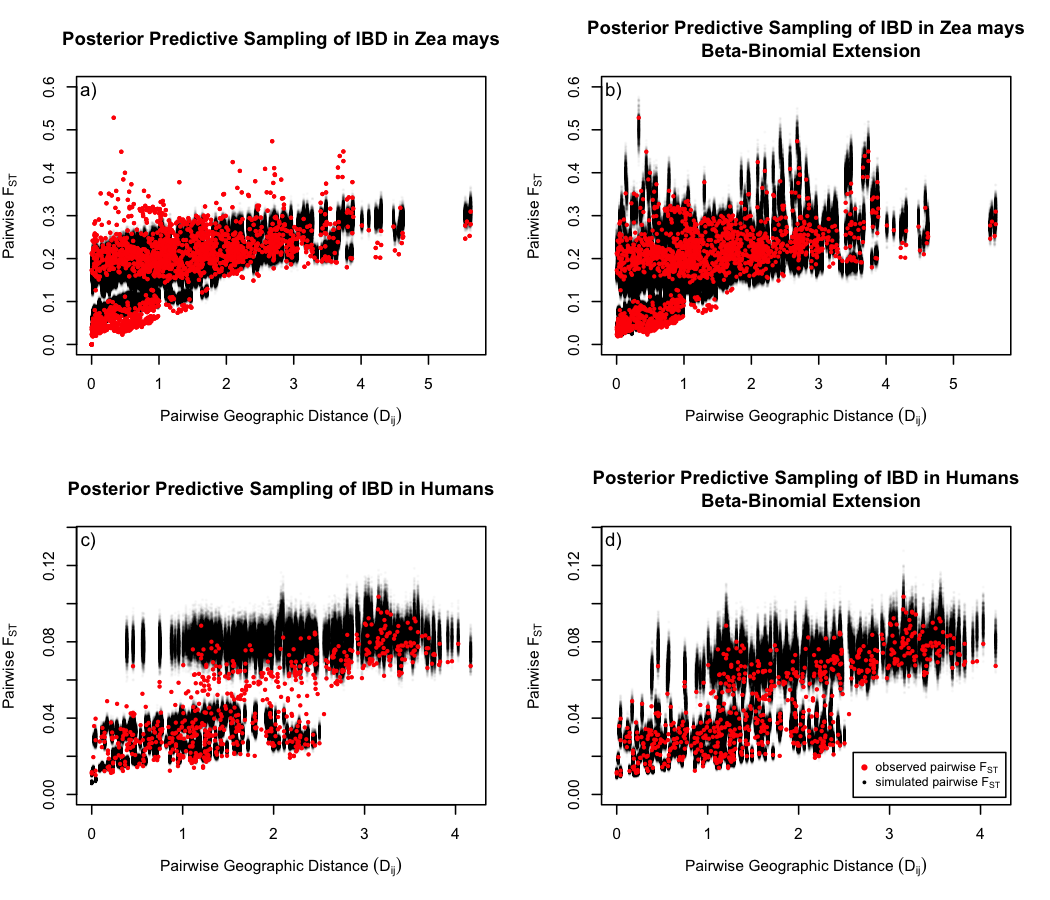
\includegraphics[width=6in,height=5.14in]{figs/bedassle/fig_3.png}
 \caption{
 		\textmd{Posterior predictive sampling with 1,000 simulated datasets, using pairwise $F_{ST}$ as a summary statistic of the allelic count data for:}
	\bf{a)}
 		\textmd{the teosinte dataset, using the standard model;}
	\bf{b)}
 		\textmd{the teosinte dataset, using the overdispersion model;}
	\bf{c)}
 		\textmd{HGDP dataset, standard model.}
	\bf{d)}
 		\textmd{HGDP dataset, overdispersion model.}
 \label{sfig:pps}
  }
\end{center}
\end{figure}
	
\subsection*{HGDP results}  
For the human (HGDP) SNP dataset analysis, the mean posterior $\alpha_{E} : \alpha_{D}$ ratio was $5.13 \times 10^{4}$, the median was $5.00 \times10^{4}$, and the 95\% credible set was $3.09 \times10^{4}$ to $7.85\times10^{4}$ (see Figure \ref{sfig:him_traceplot}\textit{a}). However, this result seems to be sensitive to outlier populations, as the beta-binomial extension of this method on the same dataset yields significantly different results, with a mean $\alpha_{E} : \alpha_{D}$ ratio of $1.35\times10^{4}$, a median of $1.34\times10^{4}$, and a 95\% credible set from $1.09\times10^{4}$ to $1.65\times10^{4}$ (see Figure \ref{sfig:him_traceplot}\textit{b}). 
This latter result is broadly consistent with that of \citet{Rosenberg2011}, who found an effect size ratio of $9.52\times10^{3}$ in a linear regression analysis that treated pairwise population comparisons as independent observations. The interpretation of our result is that being on the opposite side of the Himalaya mountain range has the impact of between approximately 11 and 16 thousand kilometers of extra pairwise geographic distance on  genetic differentiation. 

Under our beta-binomial extension values of $F_{k}$ estimated across populations ranged from $3.2 \times10^{-4}$ to 0.06.  Population values of $F_{k}$ are shown on the map in Figure \ref{sfig:him_Fk_map}. 

Posterior predictive sampling again indicates a better fit to the data including overdispersion (see Figure \ref{sfig:pps}\textit{c} and \textit{d}): the mean Pearson's product moment correlation between the posterior predictive datasets and the observed data without the beta-binomial extension was 0.88, while the mean correlation with the beta-binomial model was 0.91 (see Figure \ref{sfig:pps.corr}\textit{b}).  The ability of the model to predict specific pairwise population $F_{ST}$ is shown in Figure \ref{sfig:him.pps.pval}.  

\section*{Discussion}

In this paper, we have presented a method that uses raw allelic count data to infer the relative contribution of geographic and ecological distance to genetic differentiation between sampled populations. 
The method performs quite well: we have shown that it reliably and accurately estimates correct parameter values using simulations, and produces sensible models that give a good fit to observed patterns of differentiation in real datasets.
We feel that our method has broad utility to the field of landscape genetics and to studies of local adaptation, and holds a number of advantages over existing methods.  
(although see \citet{Wang2012} for another recent approach.)
It allows users to simultaneously quantify effect sizes of geographic distance and ecological distance (rather than assessing the significance of a correlation once the effect of geography has been removed, as in the partial Mantel test).  Explicitly modeling the covariance in allele frequencies allows users to accommodate non-independence in the data, and the method's Bayesian framework naturally accommodates uncertainty and provides a means of evaluating model adequacy.  
The inclusion of overdispersion allows fit to a set of populations with heterogeneous demographic histories.
In addition, the basic model presented here -- a parametric model of spatial covariance in allele frequencies -- is extremely versatile, allowing for the inclusion of multiple ecological or geographic distance variables, as well as great flexibility in the function used to model the covariance.  


\subsection*{Simulation Study}


Our method performed well in both simulation studies (see Figure \ref{sfig:sim_summs}, Table \ref{tab:sim_summs}, and Figure \ref{sfig:fig5_allmarg}), and was able to effectively recognize and indicate when an ecological variable contributes significantly to genetic differentiation.  This is in contrast to the partial Mantel, which has a high false positive rate in the presence of spatial autocorrelation of environmental variables (see Figure \ref{sfig:Pmantel}).

For datasets simulated under the inference model, coverage, accuracy, and precision were all satisfactory (see Table \ref{tab:sim_summs}). The precision of our estimator of $\alpha_E$ was generally lower for our discrete ecological variable, likely due to the strong spatial structure of the discrete ecological variable.  

For datasets simulated using the spatial coalescent, there were no true values for the $\alpha_{E}:\alpha_{D}$ ratio to compare with those inferred by the method.  However, we note that the $\alpha_{E}:\alpha_{D}$ ratios estimated across analyzed simulated datasets tracked the barrier effect sizes used to simulate them, and that when the barrier had no effect on migration, the marginal distributions on the $\alpha_{E}:\alpha_{D}$ ratio estimated were stacked up against the prior bound at zero and had very low median values.  The width of the 95\% credible set of the marginal posteriors grew with the barrier effect size as a result of the flattening of the posterior probability surface as true parameter value increased.  Overall, the method performed well on the datasets simulated under a model different from that used for inference (and presumably closer to reality).

An issue we observed in practice is that at some parameter values, different combinations of $\alpha$ are essentially nonidentifiable --- the form of the covariance given in equation \eqref{eqn:covariance_form} sometimes allows equally reasonable fits at different values of $\alpha_2$, or at different combinations of $\alpha_0$, $\alpha_{D}$, and $\alpha_{E}$.  
(In other cases, all four parameters can be well-estimated.)
Even when this is the case, the $\alpha_E$ : $\alpha_D$ ratio, which is the real parameter of interest,
remains constant across the credible region, even as $\alpha_E$ and $\alpha_D$ change together to compensate for changes in $\alpha_2$ and $\alpha_0$.
Such `ridges' in the likelihood surface are readily diagnosed by viewing the trace plots and joint marginals of the $\alpha$ parameters (see Figures \ref{sfig:trace_plots} and \ref{sfig:joint_marginals}).

\subsection*{Empirical Results}

\subsubsection*{Teosinte}

The application of our method to the teosinte SNP dataset indicated that difference in elevation has a potentially substantial contribution to genetic differentiation between teosinte populations.  Difference in elevation could be correlated with another, as yet unmeasured ecological variable, so we cannot claim to report a causal link, but these results are certainly suggestive, especially in the light of the research on morphological adaptations in teosinte to high altitude \citep{EaglesLothrop1994}.  

The analysis of the teosinte SNP data with the beta-binomial extension of our method shows a much better model fit, and highlights a number of populations with particularly high $F_{k}$ values.  These populations (highlighted in Figure \ref{sfig:zea_Fk_map}) all belong to the subspecies \textit{Zea mays mexicana}, which primarily occurs at higher altitudes and is hypothesized to have undergone significant drift due to small effective population sizes or bottlenecks \citep{Fukunaga2005}.  In addition, a number of these populations occur in putative hybrid zones between \textit{Zea mays mexicana} and \textit{Zea mays parviglumis}, a separate, co-occuring subspecies \citep{vanHeerwaarden2011}.  Like drift, admixture would have the effect of increasing the variance in observed allele frequencies around the expectation derived from the strict geographic/ecological distance model, and would drive up the inferred $F_{k}$ parameters for admixed populations.  

\subsubsection*{HGDP}

In the Human Genome Diversity Panel data we find a strong effect of separation by the Himalayas on genetic differentiation, confirming previous results \citep[e.g.][]{Rosenberg2005}.
To obtain a good fit to the data it is necessary to model overdispersion (with the beta-binomial extension).  This lack of model fit of the basic model can be seen in the posterior predictive sampling in Figure \ref{sfig:pps}\textit{c} and \textit{d}, which highlights the importance of assessing model adequacy during analysis. 
Under the beta-binomial extension the $\alpha_E/\alpha_D$ ratio estimates an effect of the Himalayas far greater than the distance simply to circumnavigate around the Himalayas.  We think this likely reflects the fact that Eurasian populations are away from migration-selection equilibrium, reflecting past large-scale population expansions \citep{Keinan2007}.

 With overdispersion included, the model appears to describe the data reasonably well, suggesting substantial heterogeneity beyond that dictated by geographic distance and separation by the Himalayas between the sampled populations.  A number of populations stand out in their $F_{k}$ values, in particular the Kalash, the Lahu, the Mozabites, the Hazara, and the Uygur (highlighted in Figure \ref{sfig:him_Fk_map}). This is consistent with the known history of these populations and previous work on these samples \citep{Rosenberg2002}, which suggests that these populations are unusual for their geographic position (that is, they depart from expectations of their covariance in allele frequencies with their neighbors). The Hazara and Uygur populations are known to be recently admixed populations between central Asian and East ancestry populations.  The Mozabite population has substantial recent admixture from Sub-Saharan African populations \citep{Rosenberg2002,Rosenberg2011}.  The Kalash, who live in northwest Pakistan, are an isolated population with low heterozygosity, suggesting a historically small effective population size.  Finally the Lahu have unusually low heterozygosity compared to the other East Asian populations, suggesting that they too may have had an unusually low effective population size.  Thus our beta-binomial model, in addition to improving the fit to the data, is successfully highlighting populations that are outliers from simple patterns of isolation by distance.


\subsubsection*{Population-specific variance}
As noted above, in both empirical datasets analyzed, the beta-binomial extension to the basic model offers substantially better model fit. This could in part reflect ecological variables not included in the analyses, in addition to heterogeneity in demographic processes, both of which could shape genetic variation in these populations by pushing population allele frequencies away from their expectations under our simple isolation by distance and ecology model.  Our $F_{k}$ statistic provides a useful way to highlight populations that show the strongest deviations away from our model, and to prevent these deviations from obscuring environmental correlations or causing spurious correlations.  Therefore, we recommend that the extended model be used as the default model for analyses. 

\subsection*{Limitations}
The flexibility of this statistical model is accompanied by computational expense.  Depending on the number of loci and populations in a dataset, as well as the number of MCMC generation required to accurately describe the stationary distribution, analyses can take anywhere from hours to days.  Speedups could be obtained by parallelization or porting code to C.  In addition, as with any method that employs an MCMC algorithm, users should take care to assess MCMC performance to ensure that the chain is mixing well, has been run for a sufficient number of generations, and has converged on a stationary distribution \citep{Gilks1996}.  Users are well advised to run multiple independent chains from random initial locations in parameter space, and to compare the output of those analyses to confirm that all are describing the same stationary distributions. 

Our model rests on a number of assumptions, principal among which is that population allele frequencies are well-represented by a spatially homogeneous process, such as are obtained under mutation-migration equilibrium.  That is, we assume that current patterns of gene flow between populations are solely responsible for observed patterns of genetic differentiation.  
Some examples of biological situations that may violate the assumptions of our model include: two populations that have higher genetic differentiation than expected based on their pairwise geographic distance because they arrived in nearby locations as part of separate waves of colonization;  or two populations that have been recently founded on either side of some landscape element that truly does act as a barrier to gene flow, but that do not exhibit strong genetic differentiation yet, because the system is not in equilibrium.  In reality, we expect that very few natural populations will conform perfectly to the assumptions of our model; however, we feel that the method will provide valid approximations of the patterns for many systems, and that it will be a useful tool for teasing apart patterns of genetic variation in populations across heterogeneous landscapes.

\subsection*{Extensions}

The flexibility of this method translates well into extendability.  Among a number of natural extensions the community might be interested in implementing, we highlight a few here.  

One natural extension is to incorporate different definitions of the ecological distance between our populations. 
Just because two populations have no difference in their ecological variable state does not guarantee that there is not great heterogeneity in the distance between them.  For example, a pair of populations separated by the Grand Canyon might have nearly identical elevations, but the cost to migrants between them incurred by elevation may well be significant.  
One solution to this would be to enter a simple binary barrier variable, or
to calculate least-cost paths between populations, and use those distances in lieu of geographic distance.  
A more elegant solution would be to use ``isolation by resistance'' distances,
obtained by rasterizing landscapes and employing results relating mean passage rates of random walks in a heterogeneous environment to quantities from circuit theory in order to calculate the conductance (ease of migration) between nodes on that landscape \citep{McRaeBeier2007}.  This method has the advantage of integrating over all possible pathways between populations.
Currently, users must specify the resistance of landscape elements \emph{a priori}, but those resistance parameters could be incorporated into our parametric covariance function, and estimated along with the other parameters of our model in the same MCMC.  This approach carries great appeal, as it combines the conceptual rigor of accommodating multiple migration paths with the methodological rigor of statistically estimated, rather than user-specified, parameter values.  

Another extension is the further relaxation of the assumption of process homogeneity in decay of allelic covariance over geographic and ecological distance.  Specifically, the method currently requires that a single unit of pairwise ecological distance translate into the same extent of pairwise genetic differentiation between all population pairs.  This assumption is unlikely to be realistic in most empirical examples, especially if populations are locally adapted.  For example, individuals from populations adapted to high elevation may be able to migrate more easily over topography than individuals from populations adapted to low elevations.  Such heterogeneity could be accommodated by using different covariance functions for different, pre-specified population pairings.  

A final extension that could be integrated into this method is a model selection framework, in which models with and without an ecological distance variable, or with different combinations of ecological distance variables, can be rigorously compared. 
Because our method is implemented in a Bayesian framework, we could select between models by calculating Bayes factors (the ratio of the marginal likelihoods of the data under two competing hypotheses) \citep{Dickey1971, VerdinelliWasserman1995}.  
This approach would seem to offer the best of both worlds: robust parameter inference that accommodates uncertainty in addition to output that could be interpreted as definitive evidence for or against the association of an ecological variable of interest with genetic differentiation between populations.  

\subsection*{Conclusion}

In closing, we present a tool that can be useful in a wide variety of contexts,
allowing a description of the landscape as viewed by the movements of genetic material between populations.
We urge users to be cautious in their interpretation of results generated with this model.  A correlation between genetic differentiation and an ecological distance variable does not guarantee a causal relationship, especially because unmeasured ecological variables may be highly correlated with those included in an analysis.  In addition, evidence of a correlation between genetic differentiation and an ecological variable may not be evidence of local adaptation or selection against migrants, as both neutral and selective forces can give rise to an association between genetic divergence and ecological distance.  

Finally, we are making this method available online at \textit{genescape.org}, and we hope that users elaborate on the framework we present here to derive new models that are better able to describe empirical patterns of isolation by distance --- both geographic and ecological.  


%\subsection*{Acknowledgements}
%We thank Yaniv Brandvain, Marjorie Weber, Luke Mahler, Will Wetzel, B. Moore and the Coop lab for their counsel, Jeff Ross-Ibarra and Torsten G\"{u}nther for their help with empirical datasets,  J. Novembre and D. Davison for their code, and Jon Wilkins and two anonymous reviewers for their comments on previous drafts.  
%This material is based upon work supported by the National Science Foundation under Grant No. 1262645 (PR and GC), NSF GRFP No. 1148897 (GB), a NIH Ruth L. Kirschstein NRSA fellowship F32GM096686 (PR), and a Sloan Foundation fellowship (GC). 

\clearpage
\section*{Appendix}
\subsection*{Priors}
We denote a gamma distribution with given shape and rate parameters as $\Gamma(\mbox{shape},\mbox{rate})$, a normal distribution with given mean and variance parameters as $N(\mbox{mean},\mbox{variance})$, an exponential distribution with given rate parameter $\Exp(\mbox{rate})$, and a uniform distribution between given upper and lower boundaries as $U(\mbox{lower},\mbox{upper})$.  The priors specified on the parameters of this model are: $\alpha_{0} \sim \Gamma(0.001,0.001)$; $\alpha_{D} \sim \Exp(1)$; $\alpha_{E} \sim \Exp(1)$; $\alpha_{2} \sim U(0.1,2)$; and $\mu_{\ell} \sim N(0,1/\beta)$, with a hyper-prior $\beta \sim \Gamma(0.001,0.001)$.

The priors on $\alpha_D$ and $\alpha_E$ were chosen to reflect the assumption that there is some, and potentially very great, effect of isolation by geography and ecology.  The priors on $\alpha_2$, $\alpha_0$, and $\beta$ were the same as those used by \citep{Wasser2004}, and, in the case of the latter two (on $\beta$ and $\alpha_0$), were chosen because they were conjugate to the likelihood, so their parameters could therefore be updated by a Gibbs sampling step.  

In early implementations of our method, we experimented with uniform priors on  $\alpha_D$ and $\alpha_E$ (U(0,4)), as used by \citet{Wasser2004} (although they did not have a parameter analogous to $\alpha_E$).  We replaced these uniform priors with exponentials to reflect the fact that we have no prior belief that there should be any upper bound to the effects geographic or ecological distance may have on genetic differentiation.  In practice, we found that for all simulated and empirical datasets tested, there was sufficient information in the data for the likelihood function to swamp the effect of the priors --- whether uniform or exponential --- on $\alpha_D$ and $\alpha_E$.    

However, in all analyses, we encourage users to visualize the marginal distributions of each parameter at the end of a run and compare it to its prior.  If the marginal distribution looks exactly like the prior, there may be insufficient information in the data to parameterize the model effectively, and the prior may be having an unduly large impact on analysis.  If the marginal distribution for a parameter shows that it is ``piling up" against its prior's hard bound (e.g., the marginal distribution on $\alpha_E$ has a median of 1e-3, close to its hard bound at 0), that may suggest that the current form of the prior is not describing the natural distribution of the parameter for that particular dataset well (e.g., $\alpha_E$ ``wants" to be zero, but the prior is constraining it).  In both cases (the marginal posterior and the prior have significant overlap; the prior is exhibiting an edge effect), we suggest that the user experiment with different priors and/or model parameterizations to see what effect they are having on inference.

\subsection*{MCMC}
Our MCMC scheme proceeds as follows.  The chain is initiated at maximum likelihood estimates (MLEs) for $\theta$ and $\mu$, and, for  $\alpha_{0},\alpha_{D},\alpha_{E},$ and $\alpha_{2}$, at values drawn randomly from their priors.  The multiplicative inverse of the empirical variance of the MLEs of $\mu$ is used as the initial value of $\beta$.

In each generation one of $\{\mu,\beta,\theta,\alpha_{0},\alpha_{D},\alpha_{E},\alpha_{2}\}$ is selected at random to be updated. 

The priors on $\beta$ and $\alpha_{0}$ are conjugate to their marginal posteriors, and each is updated via a Gibbs sampling step.  The updated value of $\beta$ given the current $\mu$ is drawn from 
\begin{equation}
\beta \; | \; \mu_{1},\cdots,\mu_{L}  \sim \Gamma \left(0.001+\frac{L}{2},~0.001+\frac{1}{2}\sum\limits_{\ell=1}^{L}\mu_{\ell}^2 \right),
\end{equation}
and the updated value of $\alpha_{0}$ conditional on the current set of $\theta$ is drawn from 
\begin{equation}
\alpha_0 \; | \; \theta_{1},\cdots,\theta_{L} \sim \Gamma \left(1+\frac{Lk}{2}, ~1+\frac{1}{2}\sum\limits_{\ell=1}^{L}\theta_{\ell,k}\chi^{-1}\theta_{\ell,k}^{T} \right),
\end{equation}
where $k$ is the number of populations sampled, $L$ is the number of loci sequenced, and $\chi = \alpha_{0}\Omega = \exp{(-(\alpha_{D}D_{i,j}+\alpha_{E}E_{i,j})^{\alpha_{2}}})$.

The remaining parameters are updated by a Metropolis-Hastings step;
here we describe the proposal mechanisms.
The proposed updates to $\theta$ do not affect each other, and so are accepted or rejected independently.  Following Wasser \textit{et al.}~(2004) (derived from \citep{ChristensenWaagepetersen2002, Moller1998}), the proposal is chosen as $\theta_{\ell}^{'} = \theta_{\ell} +  R_{\ell}Z$, where $R$ is a vector of normally distributed random variables with mean zero and small variance (controlled by the scale of the tuning parameter on $\theta$) and $Z$ is the Cholesky decomposition of $\Omega$ (so that $ZZ^{T} = \Omega$).  Under this proposal mechanism, proposed updates to $\theta_{\ell}$ tend to stay within the region of high posterior probability, so that more updates are accepted and mixing is improved relative to a scheme in which the $\theta$ in each population were updated individually.  

Updates to $\alpha_{D}$, $\alpha_{E}$, and $\alpha_{2}$ are accomplished via a random-walk sampler (adding a normally distributed random variable with mean zero and small variance to the current value) \citep{Gilks1996}.  Updates to elements of $\mu_{\ell}$ are also accomplished via a random-walk sampler, and again the updates to each locus are accepted or rejected independently.  

In the overdispersion model, initial values of $\Phi_{k}$ are drawn from the prior for each population.  Updates are proposed one population at a time via a random-walk step, and are accepted or rejected independently.  

Well-suited values of tuning parameters (variances in the proposal distributions for $\mu,\theta,\alpha_{D},\alpha_{E}$, and $\alpha_{2}$)
and the number of generations required to accurately describe the joint posterior will vary from dataset to dataset, and so may require tuning.

%\newpage
%\bibliography{bedassle}



\clearpage

\section*{Supplemental material}
\renewcommand{\thefigure}{S1.\arabic{figure}}
\setcounter{figure}{0}
\renewcommand{\thetable}{S1.\arabic{table}}
\setcounter{table}{0}

\begin{figure}[ht!]
\begin{center}
  \includegraphics[width=6in,height=4in]{figs/bedassle/suppmat_fig1.pdf}
 \caption{
 		\textmd{Distribution of Pearson's correlations between each posterior predictive simulated dataset and the observed data, highlighting the improved fit of the overdispersion model to describe:}
	\bf{a)}
 		\textmd{the teosinte dataset;}
	\bf{b)}
 		\textmd{the HGDP dataset.}
 \label{sfig:pps.corr}
  }
\end{center}
\end{figure}

\begin{figure}[ht!]
\begin{center}
  \includegraphics[width=6in,height=4.29in]{figs/bedassle/suppmat_fig2.pdf}
 \caption{
\textmd{Map of teosinte populations sampled, colored by their median estimated population-specific overdispersion parameter, $F_{k}$.  The five populations with the highest values are noted.}
 \label{sfig:zea_Fk_map}
  }
\end{center}
\end{figure}

\begin{figure}[ht!]
\begin{center}
  \includegraphics[width=6in,height=3.4in]{figs/bedassle/suppmat_fig3.pdf}
 \caption{
\textmd{Map of human populations included in the analysis, colored by their median estimated population-specific overdispersion parameter, $F_{k}$.  The five populations with the highest values are noted.  
The dashed line denotes the line of longitude used to delimit the Himalayas.}
 \label{sfig:him_Fk_map}
  }
\end{center}
\end{figure}

\begin{figure}[ht!]
\begin{center}
  \includegraphics[width=6in,height=4in]{figs/bedassle/suppmat_fig4.pdf}
 \caption{
 		\textmd{Histograms of p-values produced by the partial Mantel test (with 1,000,000 permutations) on the 140 datasets for which the true contribution of ecological distance to genetic differentiation was zero. The black column indicates the type I error rate with a significance level of p=0.05 in:}
	\bf{a)}
 		\textmd{the datasets with a continuous ecological distance variable;}
	\bf{b)}
 		\textmd{the datasets with a binary ecological distance variable.}
	\bf{c)}
 		\textmd{the datasets simulated under the spatial coalescent with a barrier that had no effect on genetic differentiation.}		
 \label{sfig:Pmantel}
  }
\end{center}
\end{figure}

\begin{figure}[ht!]
\begin{center}
  \includegraphics[width=5.25in,height=7in]{figs/bedassle/trace_plots.pdf}
 \caption{
 		\textmd{Trace plots of the $\alpha$ parameters of the covariance matrix $\Omega$.  Note the partial non-identifiability of the separate $\alpha$ parameters compared to the stability of the joint parameter, the $\alpha_E:\alpha_D$ ratio.}
 \label{sfig:trace_plots}
 }
\end{center}
\end{figure}

\begin{figure}[ht!]
\begin{center}
  \includegraphics[width=5.25in,height=7in]{figs/bedassle/joint_marginals.pdf}
 \caption{
 		\textmd{Joint marginal plots of the $\alpha$ parameters of the covariance matrix $\Omega$, colored by the MCMC  generation in which they were sampled.}
 \label{sfig:joint_marginals}
  }
\end{center}
\end{figure}

\begin{figure}[ht!]
\begin{center}
  \includegraphics[width=5.25in,height=7in]{figs/bedassle/acceptance_rates.pdf}
 \caption{
 		\textmd{Acceptance rates for the parameters of the model that are updated with random-walk samplers, plotted over the duration of an individual MCMC run.  Dashed green lines indicate the bounds of acceptance rates that indicate optimal mixing: 20\%-70\%.}
 \label{sfig:acceptance_rates}
  }
\end{center}
\end{figure}


\begin{figure}[ht!]
\begin{center}
  \includegraphics[width=6in,height=3.4in]{figs/bedassle/suppmat_fig5.pdf}
 \caption{
		\textmd{Heatmapped matrices showing the performance of the model at all pairwise population comparisons.  The posterior predictive p-value was defined as 
		$1-2 \times |0.5-ecdf(F_{ST_{obs}})|$, in which $ecdf(F_{ST_{obs}})$ is the empirical cumulative probability of the observed $F_{ST}$ between two populations from a distribution defined by the posterior predictive sample for that population comparison, representing the p-value of a two-tailed t-test.  Higher p-values indicate better model fit.  Populations are enumerated on the margins, and may be referenced in SuppMat Table 1.1.}
	\bf{a)}
 		\textmd{The standard model.}
	\bf{b)}
 		\textmd{The overdispersion model.}
 \label{sfig:zea.pps.pval}
  }
\end{center}
\end{figure}

\begin{figure}[ht!]
\begin{center}
  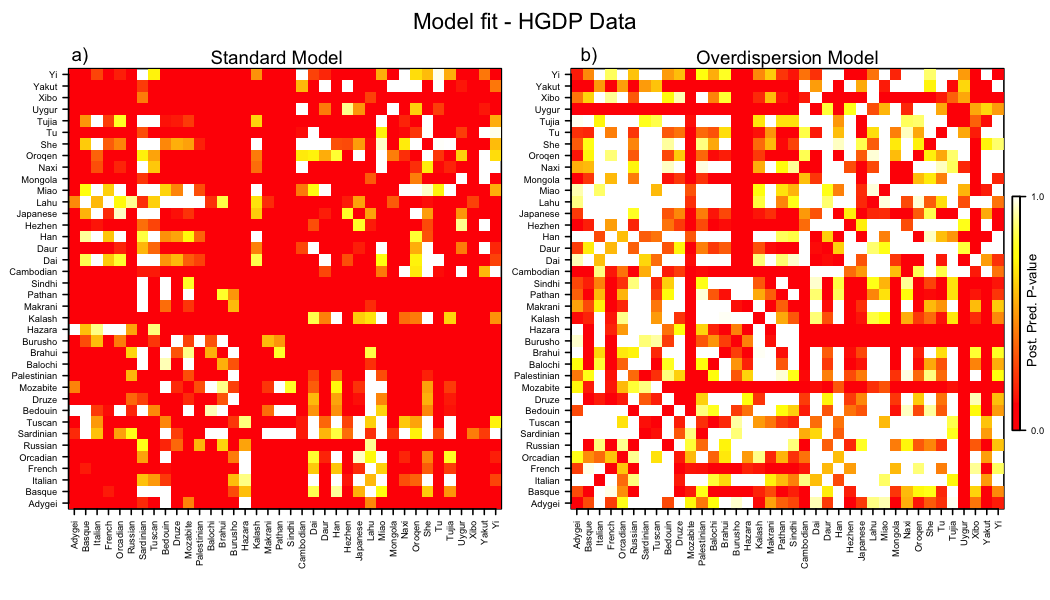
\includegraphics[width=6in,height=3.4in]{figs/bedassle/suppmat_fig6.png}
 \caption{
\textmd{Heatmapped matrices indicating the performance of the model at all pairwise population comparisons.  The posterior predictive p-value was defined as 
		$1-2 \times |0.5-ecdf(F_{ST_{obs}})|$, in which $ecdf(F_{ST_{obs}})$ is the empirical cumulative probability of the observed $F_{ST}$ between two populations from a distribution defined by the posterior predictive sample for that population comparison, representing the p-value of a two-tailed t-test.  Higher p-values indicate better model fit.  Populations are enumerated on the margins, and may be referenced in SuppMat Table 1.2.}
	\bf{a)}
 		\textmd{The standard model.}
	\bf{b)}
 		\textmd{The overdispersion model.}
\label{sfig:him.pps.pval}
  }
\end{center}
\end{figure}

\begin{figure}[ht!]
\begin{center}
  \includegraphics[width=4.66in,height=2.66in]{figs/bedassle/suppmat_fig7a.pdf}
  \includegraphics[width=4.66in,height=2.66in]{figs/bedassle/suppmat_fig7b.pdf}  
 \caption{
\textmd{Trace plots of the marginal posterior estimates for the $\alpha_{E} / \alpha_{D}$ ratio from MCMC analysis of the teosinte dataset.  Inset figures 
		give the marginal densities and 95\% credible set for the samples after a burn-in of 20\%}
	\bf{a)}
 		\textmd{The standard model.}
	\bf{b)}
 		\textmd{The overdispersion model.}
\label{sfig:zea_traceplot}
  }
\end{center}
\end{figure}


\begin{figure}[ht!]
\begin{center}
  \includegraphics[width=4.66in,height=2.66in]{figs/bedassle/suppmat_fig7c.pdf}
  \includegraphics[width=4.66in,height=2.66in]{figs/bedassle/suppmat_fig7d.pdf}  
 \caption{
\textmd{Trace plots of the marginal posterior estimates for the $\alpha_{E} / \alpha_{D}$ ratio from MCMC analysis of the HGDP dataset.  Inset figures 
		give the marginal densities and 95\% credible set for the samples after a burn-in of 20\%}
	\textbf{a)}
 		The standard model.
	\textbf{b)}
 		The overdispersion model.
\label{sfig:him_traceplot}
  }
\end{center}
\end{figure}


\begin{table}
\begin{center}
\tiny{
    \begin{tabular}{r@{--}lllll}
  \hline
  & Population name (sample size) & Latitude & Longitude & Elevation & Subspecies \\ 
  \hline
1 & Km 1 El Crustel-Teloloapan (44) & 18.383 & 18.383 & 985 & parviglumis \\ 
2 & Amates Grandes (50) & 18.388 & 18.388 & 1110 & parviglumis \\ 
3 & Km 3 Amates Grandes-Teloloapan (48) & 18.394 & 18.394 & 1210 & parviglumis \\ 
4 & Km 72 Iguala-Arcelia (Km Alcholoa-Arcelia) (56) & 18.414 & 18.414 & 1506 & parviglumis \\ 
5 & Rinc\'on del Sauce (56) & 18.35 & 18.35 & 1624 & parviglumis \\ 
6 & Ahuacatitl\'an (km 1.5 del entronque) (38) & 18.356 & 18.356 & 1528 & parviglumis \\ 
7 & Km 80 Huetamo-Villa Madero (50) & 19.063 & 19.063 & 832 & parviglumis \\ 
8 & Puerto de la Cruz (Km 119 Huetamo-V.Madero) (40) & 18.963 & 18.963 & 870 & parviglumis \\ 
9 & El Zapote (km 122 Huetamo-Caracuaro) (50) & 18.938 & 18.938 & 915 & parviglumis \\ 
10 & Puerto El Coyote (40) & 18.916 & 18.916 & 727 & parviglumis \\ 
11 & Km 135-136 Huetamo-Villa Madero (40) & 18.9 & 18.9 & 677 & parviglumis \\ 
12 & Cuirindalillo (km 142 Huetamo-Caracuaro) (42) & 18.883 & 18.883 & 697 & parviglumis \\ 
13 & Crucero Puertas de Chiripio (50) & 18.794 & 18.794 & 653 & parviglumis \\ 
14 & Quenchendio (km 151.5 Zit\'acuaro-Huetamo) (54) & 18.805 & 18.805 & 635 & parviglumis \\ 
15 & El Potrero (km 145.5 Zit\'acuaro-Huetamo) (40) & 18.82 & 18.82 & 654 & parviglumis \\ 
16 & La Crucita (km 135 Zit\'acuaro-Huetamo) (58) & 18.858 & 18.858 & 609 & parviglumis \\ 
17 & El Guayabo (km 132.5 Zit\'acuaro-Huetamo) (54) & 18.862 & 18.862 & 555 & parviglumis \\ 
18 & Km 107-108 Toluca-Altamirano (50) & 18.899 & 18.899 & 1422 & parviglumis \\ 
19 & Km 112 Toluca-Altamirano (46) & 18.895 & 18.895 & 1355 & parviglumis \\ 
20 & Km 119 Toluca-Altamirano (38) & 18.854 & 18.854 & 1015 & parviglumis \\ 
21 & Salitre-Monte de Dios (46) & 18.842 & 18.842 & 958 & parviglumis \\ 
22 & Taretan (La Perimera) (36) & 19.344 & 19.344 & 1170 & parviglumis \\ 
23 & Los Guajes (km 43 Zit\'acuaro-Huetamo) (54) & 19.231 & 19.231 & 985 & parviglumis \\ 
24 & 1 Km Norte de Santa Ana (54) & 19.281 & 19.281 & 1332 & parviglumis \\ 
25 & Km 8 Zuluapan-Tingambato (58) & 19.148 & 19.148 & 1178 & parviglumis \\ 
26 & Km 4 Zuluapan-Tingambato (60) & 19.146 & 19.146 & 1346 & parviglumis \\ 
27 & K2 Zacazonapan-Otzoloapan (56) & 19.079 & 19.079 & 1468 & parviglumis \\ 
28 & K22 Zacazonapan-Luvianos (EL Puente) (56) & 19.039 & 19.039 & 1085 & parviglumis \\ 
29 & Acatitl\'an-El Puente (50) & 19.029 & 19.029 & 1075 & parviglumis \\ 
30 & Queretanillo (56) & 19.551 & 19.551 & 1342 & parviglumis \\ 
31 & Km 33.5 Temascal-Huetamo (56) & 19.483 & 19.483 & 1100 & parviglumis \\
32 & Km 37 Temascal-Huetamo (40) & 19.464 & 19.464 & 1030 & parviglumis \\ 
33 & Casa Blanca (km 62 Huetamo-Villa Madero) (54) & 19.161 & 19.161 & 1268 & parviglumis \\  
   \hline
\end{tabular}
}
\label{tab:zea_popdata1}
\end{center}
\caption{Metadata for \textit{Z. m. parviglumis} populations used in the teosinte dataset.}
\end{table}

\begin{table}
\begin{center}
\tiny{
    \begin{tabular}{r@{--}lllll}
  \hline
  & Population name (sample size) & Latitude & Longitude & Elevation & Subspecies \\ 
  \hline
34 & San Antonio Tecomitl (4) & 19.217 & 19.217 & 2400 & mexicana \\ 
35 & Ozumba (4) & 19.05 & 19.05 & 2340 & mexicana \\ 
36 & Temamatla (6) & 19.183 & 19.183 & 2400 & mexicana \\ 
37 & Zoquiapan (4) & 19.317 & 19.317 & 2270 & mexicana \\ 
38 & Los Reyes La Paz (6) & 19.4 & 19.4 & 2200 & mexicana \\ 
39 & Miraflores (4) & 19.217 & 19.217 & 2200 & mexicana \\ 
40 & Tepetlixpa (4) & 19.017 & 19.017 & 2320 & mexicana \\ 
41 & El Pedregal (4) & 19.267 & 19.267 & 2500 & mexicana \\ 
42 & Mexicaltzingo (4) & 19.217 & 19.217 & 2600 & mexicana \\ 
43 & Santa Cruz (4) & 19.083 & 19.083 & 2425 & mexicana \\ 
44 & San Antonio (4) & 19.067 & 19.067 & 2440 & mexicana \\ 
45 & San Salvador (4) & 19.133 & 19.133 & 2425 & mexicana \\ 
46 & Tlachichuca (4) & 19.167 & 19.167 & 2355 & mexicana \\ 
47 & K3 San Salvador El Seco-Coatepec (4) & 19.117 & 19.117 & 2425 & mexicana \\ 
48 & San Nicolas B. Aires (4) & 19.167 & 19.167 & 2355 & mexicana \\ 
49 & San Felipe (4) & 19.517 & 19.517 & 2250 & mexicana \\ 
50 & 4 miles N of Hidalgo, Arroyo Zarco (4) & 19.7 & 19.7 & 2040 & mexicana \\ 
51 & 5-7 km SW Cojumatlan (4) & 20.1 & 20.1 & 1700 & mexicana \\ 
52 & Puente Gavilanes (4) & 24.017 & 24.017 & 1950 & mexicana \\ 
53 & La Estancia (4) & 21.5 & 21.5 & 1920 & mexicana \\ 
54 & Moroleon (4) & 20.083 & 20.083 & 2100 & mexicana \\ 
55 & Pinicuaro (8) & 20.05 & 20.05 & 2087.5 & mexicana \\ 
56 & Puruandiro (4) & 20.083 & 20.083 & 2000 & mexicana \\ 
57 & km 2 Puruandiro-Las Tortugas (4) & 20.117 & 20.117 & 1880 & mexicana \\ 
58 & 10 km S of Degollado (4) & 20.367 & 20.367 & 1625 & mexicana \\ 
59 & Ayotlan (4) & 20.417 & 20.417 & 1520 & mexicana \\ 
60 & Churitzio (8) & 20.175 & 20.175 & 1780 & mexicana \\ 
61 & El Salitre 1-2 km SE (4) & 20.183 & 20.183 & 1530 & mexicana \\ 
62 & Rancho El Tejocote (4) & 20.167 & 20.167 & 1750 & mexicana \\ 
63 & Villa Escalante (6) & 19.4 & 19.4 & 2320 & mexicana \\ 
   \hline
\end{tabular}
}
\label{tab:zea_popdata2}
\end{center}
\caption{Metadata for \textit{Z. m. mexicana} populations used in the teosinte dataset.}
\end{table}


\begin{table}
\begin{center}
\tiny{
    \begin{tabular}{r@{--}lccc}
  \hline
  & Population name (sample size) & Latitude & Longitude & Side of the Himalayas \\ 
  \hline
1 & Adygei (30) & 44 & 39 & W \\ 
2 & Basque (36) & 43 & 0 & W \\ 
3 & Italian (20) & 46 & 10 & W \\ 
4 & French (52) & 46 & 2 & W \\ 
5 & Orcadian (28) & 59 & -3 & W \\ 
6 & Russian (46) & 61 & 40 & W \\ 
7 & Sardinian (46) & 40 & 9 & W \\ 
8 & Tuscan (10) & 43 & 11 & W \\ 
9 & Bedouin (86) & 31 & 35 & W \\ 
10 & Druze (78) & 32 & 35 & W \\ 
11 & Mozabite (50) & 32 & 3 & W \\ 
12 & Palestinian (88) & 32 & 35 & W \\ 
13 & Balochi (44) & 30.5 & 66.5 & W \\ 
14 & Brahui (46) & 30.5 & 66.5 & W \\ 
15 & Burusho (48) & 36.5 & 74 & W \\ 
16 & Hazara (40) & 33.5 & 70 & W \\ 
17 & Kalash (44) & 36 & 71.5 & W \\ 
18 & Makrani (48) & 26 & 64 & W \\ 
19 & Pathan (40) & 33.5 & 70.5 & W \\ 
20 & Sindhi (44) & 25.5 & 69 & W \\ 
21 & Cambodian (16) & 12 & 105 & E \\ 
22 & Dai (18) & 21 & 100 & E \\ 
23 & Daur (14) & 48.5 & 124 & E \\ 
24 & Han (64) & 32.5 & 114 & E \\ 
25 & Hezhen (16) & 47.5 & 133.5 & E \\ 
26 & Japanese (50) & 38 & 138 & E \\ 
27 & Lahu (12) & 22 & 100 & E \\ 
28 & Miao (10) & 28 & 109 & E \\ 
29 & Mongola (18) & 48.5 & 119 & E \\ 
30 & Naxi (14) & 26 & 100 & E \\ 
31 & Oroqen (16) & 50.5 & 126.5 & E \\ 
32 & She (18) & 27 & 119 & E \\ 
33 & Tu (18) & 36 & 101 & E \\ 
34 & Tujia (18) & 29 & 109 & E \\ 
35 & Uygur (18) & 44 & 81 & E \\ 
36 & Xibo (16) & 43.5 & 81.5 & E \\ 
37 & Yakut (46) & 63 & 129.5 & E \\ 
38 & Yi (18) & 28 & 103 & E \\ 
   \hline
\end{tabular}
}
\label{tab:hgdp_popdata}
\end{center}
\caption{Metadata for populations used from the HGDP dataset.}
\end{table}
 %This looks for chapter1.tex

% chapter 2
\chapter{Isolation by Environment}
%This is an example for a chapter, additional chapter can be added in the skeleton-thesis
%To generate the final document run latex, build and quick build commands on the skeleton-thesis file not this one.
%\chapter{Isolation by Environment}
\section*{Authors and Affiliations}
\begin{flushleft}
Ian J. Wang\textsuperscript{1},\\
Gideon S. Bradburd\textsuperscript{2},\\
\bf{1} Department of Environmental Science, Policy, and Management, University of California, Berkeley, CA
\\
\bf{2} Center for Population Biology, Department of Evolution and Ecology, University of California, Davis, CA, USA
\\
\bf{*} The authors contributed equally to this manuscript.
\end{flushleft}
%\section*{Abstract}
%The interactions between organisms and their environments can shape distributions of spatial genetic variation, resulting in patterns of isolation by environment (IBE) in which genetic and environmental distances are positively correlated, independent of geographic distance.  IBE represents one of the most important patterns that results from the ways in which landscape heterogeneity influences gene flow and population connectivity, but it has only recently been examined in studies of ecological and landscape genetics.  Nevertheless, the study of IBE presents valuable opportunities to investigate how spatial heterogeneity in ecological processes, agents of selection, and environmental variables contributes to genetic divergence in nature.  New and increasingly sophisticated studies of IBE in natural systems are poised to make significant contributions to our understanding of the role of ecology in genetic divergence and of modes of differentiation both within and between species.  Here, we describe the underlying ecological processes that can generate patterns of IBE, examine its implications for a wide variety of disciplines, and outline several areas of future research that can answer pressing questions about the ecological basis of genetic diversity.
\renewcommand{\thefigure}{2.\arabic{figure}}
\setcounter{figure}{0}
\renewcommand{\thetable}{2.\arabic{table}}
\setcounter{table}{0}

\section*{Introduction}
	Seventy-one years ago, Sewall Wright \citep{Wright1943} introduced the term ``isolation by distance" (IBD) to describe a pattern in which genetic differentiation at neutral loci increases with geographic distance.  The theory of isolation by distance describes the local accumulation of genetic differences when dispersal between populations or subgroups is geographically restricted \citep{Slatkin_1993}.  Effectively, neutral genetic differentiation between populations is the result of drift acting within populations more quickly than it is ameliorated by gene flow between populations \citep{Slatkin_1993, Rousset_1997}. Therefore, any processes that reduce the effective dispersal rate between populations will generate patterns of greater genetic differentiation \citep{Slatkin_1993,Bolnick_Otto_2013}.
	Decades of investigation into IBD have revealed it to be common in nature \citep{Slatkin_1993, Meirmans_2012} and brought a focus to the geography of population divergence and isolation \citep{Mayr_1963}.  However, geography represents only one of the key landscape components that can potentially influence gene flow and population connectivity \citep{Crispo_etal_2006, Lee_Mitchell-Olds_2011}.  Another important part of a landscape is the environment \citep{Nosil_etal_2005, Foll_Gaggiotti_2006, Thorpe_etal_2008}, and in the past decade, new fields like landscape genetics \citep{Storfer_etal_2007, Balkenhol_etal_2009, Wagner_Fortin_2013} have arisen to examine the roles played by ecology and the environment in microevolutionary processes \citep{McRae_Beier_2007, Rasanen_Hendry_2008, Bolnick_Otto_2013}.  One of the important concepts that has emerged is �isolation by environment� (IBE; \cite{Wang_Summers_2010}, which encapsulates the relationship between environmental heterogeneity and spatial variation in gene flow on a landscape \citep{Wang_etal_2013,Bradburd_etal_2013,Sexton_etal_2014}.
We define isolation by environment as a pattern in which genetic differentiation increases with environmental differences, independent of geographic distance, and which is agnostic with respect to the underlying processes that generated it.  The study of IBE comprises two challenges.  The first is to disentangle the relative strengths of IBD and IBE in observed patterns of spatial genetic differentiation, which can be a difficult statistical problem because geographic distance and environmental differences are often correlated (Fig.\ \ref{sfig:ibde}; \cite{Lee_Mitchell-Olds_2011, Wang_2013, Shafer_Wolf_2013, Bradburd_etal_2013}).  The second is then to determine the processes that have generated and maintained those patterns.  The development of new methods in spatial statistics and the rapid proliferation of both genomic and environmental GIS data have greatly facilitated research to overcome the first challenge of quantifying IBE relative to IBD, but researchers seeking to tease apart these patterns must still take care to employ appropriate study design, sampling strategies, and statistical techniques \citep{Bradburd_etal_2013,Sexton_etal_2014}.  The second challenge requires assessing the ways in which drift, selection, and dispersal have acted to shape patterns of genetic variation.  Quantifying the relative contributions of these processes, the ways in which they depend upon an ecologically heterogeneous landscape, and how those relative contributions vary across species or landscapes is an active and exciting field of research.
Here, we describe the processes that can generate this pattern and discuss important methods and considerations for studying IBE.  We conclude by proposing avenues for future research in IBE and suggesting a range of new and exciting questions about the ecological basis of spatial genetic variation.  The rise of IBE as a research focus has resulted in a tremendous opportunity to examine, often at very fine scales, the ways in which ecology shapes genetic variation in nature, forming a true bridge between the fields of population genetics and landscape ecology.

\begin{figure}[ht!]
\begin{center}
  \includegraphics[width=6in,height=2.5in]{figs/ibe/IBDE_triptych.pdf}
 \caption{Isolation by distance and environment.
 Under the patterns of isolation by distance (IBD) and isolation by environment (IBE), genetic distance increases with geographic and environmental distance.  The three panels show different views of a simulated dataset in which both patterns can be seen.  Points represent the genetic distance (Gen. Dist.) between a pair of populations, plotted against their geographic (Geo. Dist.) and environmental distances (Env. Dist.), and are heat-colored by the magnitude of that environmental distance.
 \label{sfig:ibde}}
\end{center}
\end{figure}

\section*{Definition of IBE}
Isolation by environment is defined as a pattern in which genetic differentiation increases with environmental differences, independent of geographic distance \citep[Fig.\ \ref{sfig:ibde};][]{Wang_Summers_2010, Bradburd_etal_2013, Sexton_etal_2014}.  The important environmental variables may be continuous, such as elevation or humidity \citep{Murphy_etal_2010, Bradburd_etal_2013}, or discrete, such as habitat or substrate type \citep{Andrew_etal_2012}.  They may describe abiotic factors, like temperature and precipitation \citep{Wang_2012}, or biotic factors, like vegetation density and host \citep{Via_Hawthorne_2002}.  The key is that they contribute to explaining variation in pairwise genetic distances beyond that explained by geographic distance (and after accounting for any correlation between environmental and geographic distances).  This definition is solely a description of a pattern and is agnostic with respect to the processes that have generated that pattern.  
We advocate for this pattern-based, rather than process-based, definition because there are frequently many biological processes that can generate a given pattern of observed genetic differentiation.  This definition provides the general case for which numerous other �isolation by� terms present specific, process-based instances.  For example, isolation by adaptation (IBA), defined as the correlation of adaptive phenotypic and neutral genetic divergence \citep{Nosil_etal_2008}, and isolation by ecology, defined as the correlation of ecological and neutral genetic divergence \citep{Claremont_etal_2011, Edelaar_etal_2012}, both describe patterns due to a specific selective mechanism.  These process-based terms are designed to address the important question of how observed patterns of spatial genetic variation are generated; however, the processes that have generated these empirical patterns of divergence cannot be observed directly from these patterns, and the same empirical pattern of genetic differentiation could be due to many different underlying processes.
Our definition can also be contrasted with isolation by resistance (IBR), defined as the correlation of genetic and ``resistance" distances \citep{McRae_Beier_2007}.  Resistance distance between a pair of populations can be understood as the probability that an individual disperses from one to the other, integrating over all paths that individual might take, and weighting those paths by their �friction� to dispersal (a low pairwise resistance means a high probability of dispersal, and vice versa).  Isolation by resistance, like our definition of IBE, is also agnostic with respect to process; the dispersal resistance of a specific landscape element may be due to selection against maladapted dispersers, migratory preference, or simple cost of transport.  However, IBR implicitly conflates IBD and IBE, making it impossible to differentiate the strengths of these two patterns in empirical data.
Our simple but broad definition is meant to be inclusive of all positive associations between genetic and environmental distances, in keeping with the tradition set up by the definition of IBD from \citet{Wright1943}.  It provides a collective term for a genetic pattern that is common in nature but may be generated by many different processes, and it implicitly links environmental variation on a landscape to gene flow and population structure.  Thus, IBE is valuable for understanding spatial genetic differentiation in the context of landscape variation.

\section*{Processes Generating IBE}
Isolation by environment is a pattern that can be generated by a variety of ecological processes.  These may be relatively simple, like when a temperature cline regulates dispersal among populations of an ectotherm \citep[e.g.][]{Murphy_etal_2010}, or they may represent more complex ecological interactions, like when genetic differentiation between plant populations is mediated by differences in their pollinator communities \citep[e.g.][]{Hopkins_etal_2012}.  This many-to-one mapping of process to pattern can make it difficult, though by no means impossible, to learn about the mechanisms generating observed patterns of spatial genetic variation.  The first step for these investigations, and an important component for any study of IBE, is to carefully consider the potential processes that could be taking place.  Below, we identify four ecological processes � not mutually exclusive � that can generate a pattern of IBE, including (1) natural selection against immigrants, (2) sexual selection against immigrants, (3) reduced hybrid fitness, and (4) biased dispersal (Fig.\ \ref{sfig:ibe_causes}).

\begin{figure}[ht!]
\begin{center}
  \includegraphics[width=3.5in,height=3.5in]{figs/ibe/IBE_causes.pdf}
 \caption{Illustration of processes that can generate a pattern of isolation by environment.
 Dispersal between divergent environments can be reduced when (1) natural selection acts upon immigrants adapted to different environmental conditions, (2) sexual selection limits the reproductive success of immigrants with alternative traits, (3) hybrid offspring of native and immigrant parents have reduced fitness, for instance due to intermediate phenotypes, (4a) biased dispersal resulting from a genotype or phenotype leading to a dispersal preferences for particular environments, or (4b) biased dispersal resulting from a plastic natal habitat preference.
 \label{sfig:ibe_causes}}
\end{center}
\end{figure}


\subsection*{(1) Natural Selection Against Immigrants}
Natural selection can generate IBE among populations inhabiting different environments when these populations are locally adapted \citep{Nosil_etal_2005, Rasanen_Hendry_2008}.  In these cases, populations evolve traits suited to their local environments, regardless of their fitness consequences in other environments \citep{Servedio_2004, Kawecki_Ebert_2004, Nosil_etal_2005}.  Thus, native genotypes in each environment will have, on average, higher fitness than immigrant genotypes originating in different environments \citep{Servedio_2004, Kawecki_Ebert_2004}.  When individuals or populations show ecological specialization \citep{Lu_Bernatchez_1999, Via_Hawthorne_2002}, divergent natural selection will limit the reproductive success of individuals moving into different environments from which they are adapted \citep{Rasanen_Hendry_2008, Mosca_etal_2012}.  For instance, walking sticks adapted to appear cryptic on certain host plants experience greater predation from visually-oriented predators after moving to a different host species \citep{Nosil_2004, Nosil_etal_2005}, and divergent selection regimes in inland habitat with seasonal drought and coastal habitat with year round soil moisture cause nearly complete reductions in gene flow between populations of yellow monkey flowers adapted to either climate \citep{Lowry_etal_2008}.  We can expect the strength of divergent selection to be proportional to the magnitude of the differences among environments \citep{Crispo_etal_2006, Lee_Mitchell-Olds_2011, Wang_etal_2013}, and therefore, pairs of populations inhabiting increasingly different environments will experience reduced gene flow and greater genetic divergence \citep{Nosil_etal_2005, Thorpe_etal_2008}.  This environmentally associated natural selection may generate either pre- or post-mating reproductive isolation, depending on whether immigrants survive and thrive long enough to mate locally. If immigrants are able to mate locally, there may subsequently be selection against immigrant alleles in hybrids (see ``Reduced Hybrid Fitness" below). 

\subsection*{(2) Sexual Selection Against Immigrants}
Similarly, divergent sexual selection among populations inhabiting different environments can also generate IBE \citep{Servedio_2004,Nosil_etal_2005,Safran_etal_2013}.  When populations inhabiting different environments show divergence in mate choice or sexual signals, sexual selection will reduce the reproductive success of dispersers moving between them \citep{Servedio_2004, Nosil_etal_2005}.  In some cases, divergent sexual selection will be related to environmentally driven natural selection.  For instance, under the good genes hypothesis, mate choice evolves so that individuals prefer mates possessing traits that increase offspring fitness \citep{Ingleby_etal_2010}, and if the fitness conferred by these traits varies across environments, divergent sexual selection will result and lead to variation in preferences for ecologically important traits \citep{Nosil_etal_2005}.  This is the case with lesser wax moths, in which females choose males with different signals to produce offspring that mature faster in different food and temperature environments \citep{Jia_Greenfield_1997}.  In other cases, divergent sexual selection can also be related to environmental variation but not natural selection.  For instance, under the sensory drive hypothesis, sexual signals and their perception by receivers can evolve to be more effective under local environmental conditions, and therefore, dispersers may have reduced reproductive opportunities if their sexual signals are viewed in a different ecological context.  Such is the case with some cichlids \citep{Seehausen_etal_2008} and sticklebacks \citep{Boughman_2001}, in which adaptive variation in visual sensitivity leads to genetic isolation between groups expressing different nuptial coloration across gradients in ambient light conditions.  Thus, divergent sexual selection can act in concert with divergent natural selection or independently of it \citep{Servedio_2004, Nosil_etal_2005, Safran_etal_2013}, in both cases producing increased levels of IBE.  As with natural selection against immigrants, imperfect sexual selection against non-local individuals can allow for the creation of hybrid offspring, the sexual characteristics and mating behavior of which may themselves be selected against (see ``Reduced Hybrid Fitness" below).

\subsection*{(3) Reduced Hybrid Fitness}
Selection can further contribute to IBE when hybrid offspring of immigrant-native parent crosses have reduced fitness relative to their non-hybrid neighbors \citep[i.e. post-zygotic extrinsic reproductive isolation of ecologically divergent populations;][]{Nosil_etal_2005, McBride_Singer_2010}.  If hybrid offspring have intermediate phenotypes, then they may not occupy an available ecological niche in their natal environment or may have limited mating opportunities, both of which will reduce effective rates of long-term gene flow \citep{Nosil_etal_2005, Garant_etal_2007, McBride_Singer_2010}.  For instance, in Euphydryas butterflies, hybrids from parents adapted to different hosts exhibit intermediate traits that are significantly maladaptive, including foraging and oviposition behaviors \citep{McBride_Singer_2010}.  These cases will mostly serve to strengthen the patterns resulting from natural or sexual selection on immigrants.  However, we consider this separate from these processes, as other authors have \citep[e.g.][]{Servedio_2004, Nosil_etal_2005}, because selection acts on a different generation of individuals, rather than on the immigrants themselves, and under certain scenarios, the determinants of offspring fitness may be different from those of immigrant fitness.  For example, if combinations of alleles that arose in isolated parental populations are incompatible, hybrid fitness may be reduced due to intrinsic, rather than extrinsic reproductive isolation (e.g. Dobzhansky-Muller Incompatibilities, \cite{Dobzhansky1937}); in this case, selection would not be against immigrant alleles, but rather against the combination of immigrant and native alleles.

\subsection*{(4) Biased Dispersal}
Isolation by environment can also result when a genotype, phenotype, or behavior contributes to a dispersal preference for a particular environment.  Under these cases of `biased' or `directed' dispersal, an individual's traits affect the likelihood of moving to various habitats.  This may be due to heritable variation \citep{Edelaar_etal_2008, Bolnick_Otto_2013} or may be the result of a behavioral or plastic response induced by an individual�s natal or developmental environment \citep{Davis_Stamps_2004}.  A dispersal bias may arise because of a fitness or performance advantage in a particular environment, like the matching of coloration and habitat in white sand lizards \citep{Rosenblum_Harmon_2011}.  In this case, the resulting pattern of dispersal naturally leads to the correlation of genotype and environment \citep{Bolnick_Otto_2013}.  However, such a pattern may also arise even when individuals do not necessarily experience differential selection in different habitats, for instance when dispersers avoid novel habitat when moving across an environmentally heterogeneous landscape \citep{Stevens_etal_2004,Feder_Forbes_2007} or when individuals prefer to disperse to habitats similar to their native habitat, known as natal habitat preference induction \citep{Davis_Stamps_2004}.  This type of environmentally-induced plastic response can be seen in two species of true frogs, in which the exposure of eggs to olfactory cues in water led to a preference among tadpoles for those environmental cues that is maintained through metamorphosis \citep{Hepper_Waldman_1992}.  In such cases, there does not need to be local adaptation, but a pattern of IBE may still arise.  We consider these processes distinct from natural or sexual selection against immigrants because selection may not actually act upon these individuals � there are no deaths or reproductive consequences since individuals move before any selective events can occur \citep{Bolnick_Otto_2013}.

\section*{Methods and Considerations for Studying IBE}
\subsection*{Sampling Scheme}
When investigating patterns of spatial genetic variation, a researcher must design a sampling scheme that allows the study to disentangle the relative effects of geographic distance and ecological or environmental distance.  This includes two important considerations: sampling to maximize the range of observed geographic and ecological distances, and sampling to minimize the correlation between the potential explanatory variables.  By sampling over an extensive range of geographic and environmental distances, the researcher can learn about the shape of the decay of genome-wide relatedness with different distances.  For example, if patterns of IBD or IBE increase non-linearly, a researcher with a sampling scheme that includes only small distances and large distances might be unable to quantify well the shape of that curve (Fig.\ \ref{sfig:sampling}).
	Additionally, researchers must avoid a sampling scheme in which ecological and geographic distance are confounded.  For example, in the confounded sampling configuration shown in Fig.\ \ref{sfig:sampling}, significant geographic distance is strongly correlated with environmental distance, making it difficult to statistically disentangle their effects.  Instead, samples from different environments should be drawn from a mixture of populations that are geographically close and distant, and samples from within similar environments should be as well.  This will serve to reduce the association between geographic and environmental distances.  
	For both considerations � maximizing the range of sampled pairwise distances and minimizing the correlation of covariates � a limited sampling scheme could lead to uninterpretable or misleading results.  However, empirical researchers are frequently limited in their sampling effort, and are therefore forced to make compromises in the number of locations or individuals they are able collect and genotype.  When designing sampling schemes with these compromises in mind, we suggest first examining simple histograms of pairwise distances (geographic and environmental) and correlations between environmental and geographic distances under a projected sampling scheme prior to sample collection.  If necessary, adjustments to the proposed scheme can then be made to increase the diversity of pairwise distances sampled or to minimize the correlation between these variables.
	Above, we have placed an emphasis on placement and number of sampled locations, the latter of which is negatively correlated with the number of individuals per sampling location that a researcher can afford to genotype.  Increasing the number of individuals sampled per location decreases the binomial sampling noise around estimates of population allele frequencies and is therefore useful in accurately estimating pairwise population differentiation.  However, in the era of next-generation sequencing, it is possible to sequence each individual at large numbers of loci, which, assuming they are independent, serve as independent instantiations of the coalescent process.  With many sequenced loci in two populations, it is therefore possible to get good estimates of the differentiation between them, even if the sample size at each locus is small, and the estimate of differentiation is therefore noisy \citep{Patterson_etal_2006}.
In summary, researchers designing studies to investigate IBE should seek to maximize the range of geographic and environmental distances between sampled locations, minimize the correlations of those geographic and environmental covariates, and maximize the number of sampled locations even at the cost of sample size.  In all cases, the relevant question that should be kept in mind is not whether it will be possible to detect spatial genetic differentiation but whether it will be possible to distinguish a genetic pattern of IBE from the background pattern of IBD.

\begin{figure}[ht!]
\begin{center}
  \includegraphics[width=4in,height=4.5in]{figs/ibe/sampling_scheme_figure.pdf}
  %figs/ibe/sampling_scheme_figure_hires.png}
 \caption{Illustration of common pitfalls in designing a sampling scheme.
These panels show the contrasted outcomes between complete sampling and an inadequately designed sampling scheme for populations on a hypothetical landscape with environmental variation (A).  The histogram of pairwise distances (B) obtained by a poor sample design shows that this design results in obtaining pairwise distances that are not fully representative of the full set of populations.  The comparison of the environmental and geographic distances recovered under the complete and partial sampling schemes (C) shows that these distances are highly correlated under the partial sampling scheme; IBD and IBE are conflated because all comparisons over short distances are also similar in environment, and all comparisons over long distances are environmentally disparate, with no intermediate comparisons to help disentangle the relative contributions of IBD and IBE.  Finally, pairwise genetic differentiation plotted against pairwise geographic distance and colored by environmental distance (D) shows that under the partial sampling scheme, the shape of the curves for IBD and IBE are poorly estimated.
 \label{sfig:sampling}
  }
\end{center}
\end{figure}


\subsection*{Statistical Techniques}
This same question should be at the heart of the statistical techniques used to study IBE; researchers must account for IBD when attempting to quantify IBE along one or more environmental axes.  This task is inherently difficult because measures of pairwise genetic distance are non-independent, and therefore should not be modeled directly as a function of pairwise geographic or ecological distances.  The Mantel and partial Mantel tests were designed to avoid this problem of non-independence by implementing a significance test that explicitly accounts for the pairwise nature of the dependent and independent variables.  However, when the data are spatially autocorrelated, the partial Mantel has a pathological type I error rate \citep{Guillot_Rousset_2013}, as the significance procedure implicitly rejects the spatial structure of the data.
However, the question the partial Mantel was designed to answer in landscape genetics is still vital to many research programs today: what are the relative contributions to observed patterns of spatial genetic variation from geographic and ecological distances?  Recently, several new, more statistically robust methods designed to answer this question have been released.  These include methods for examining genome-wide patterns of differentiation and for investigating divergence in individual loci, both of which are important for understanding the nature of IBE.  Coupled with new techniques for treating the spatial component of genetic variation more explicitly, these provide strength and flexibility for studying IBE in almost any natural system. 
New methods for examining general patterns of genetic differentiation fall into two categories: modeling covariance in allele frequencies and matrix regression approaches.  Of the former, BEDASSLE \citep{Bradburd_etal_2013} is a Bayesian method that models the covariance in allele frequencies across the genome as a decreasing function of pairwise geographic and ecological distances.  The coefficients estimated for these pairwise distance elements can be compared to quantify the relative impact of geographic and ecological distances on patterns of genetic variation.  This method was applied to a maize dataset and revealed that 1000m of elevation difference between populations has the same effect on genetic differentiation as about 150km of horizontal distance \citep{Bradburd_etal_2013}.  Of the latter, methods based on matrix regression, including generalized dissimilarity modeling \citep[GDM;][]{Freedman_etal_2010}, structural equation modeling \citep[SEM;][]{Wang_etal_2013}, and multiple matrix regression with randomization \citep[MMRR;][]{Wang_2013} apply a regression framework to simultaneously quantify the effects of multiple distance matrices on a single response variable, typically genetic distance, using different computational methodologies.  SEM was used to infer that IBD typically contributed about twice as much to genetic divergence as IBE in 17 species of anoles and to quantify the relative contributions of individual environmental variables to IBE in those species \citep{Wang_etal_2013}.  Both sets of methods have the power to disentangle IBD and IBE, and the preferred method to be used will depend upon the data available and the question to be answered.
New techniques for dealing with genetic distances in a spatially explicit manner include those that handle continuous spatial variation and those designed to account for the spatial arrangement of population networks.  For continuous variation, LocalDiff \citep{Duforet-Frebourg_Blum_2014} uses Bayesian kriging and MEMGENE uses Moran�s eigenvector maps \citep{Galpern_etal_2014} to detect discontinuities in patterns of gene flow across a landscape, which may be associated with landscape heterogeneity and barriers to dispersal.  For population networks, the utilization of conditional genetic distances derived from population network topology can improve estimation of IBD and IBE, and can be used with phylogeographic history to separate the effects of historical and contemporary barriers to gene flow \citep{Dyer_etal_2010}.  This method was used to parse out the effects of phylogeographic history in the Sonoran desert succulent, revealing individual effects of spatial and bioclimatic variables on genetic differentiation \citep{Dyer_etal_2010}.  Both of these techniques are valuable for handling spatial genetic distance data, especially when paired with an appropriate statistical technique for disentangling IBD and IBE. 
These approaches all consider genome-wide patterns of differentiation, and are therefore designed to answer a separate set of questions from methods like Bayenv2 \citep{coop2010bayenv,G�nther_Coop_2013}, which asks whether individual SNPs are correlated with environmental variation, and spaMM \citep{Rousset_Ferdy_2014}, which is designed to account for spatial autocorrelation in the association of a genotype with some environmental variable.  The former was applied to an Atlantic herring dataset to identify loci that were strongly differentiated along a salinity gradient \citep{G�nther_Coop_2013}.  Once patterns of differentiation have been identified, additional methods can be applied to genomic data to attempt to elucidate the population-level processes that have generated those patterns.  These methods, which are principally designed to look for the signature of selection across the whole genome, include identifying signals of selective sweeps and genomic hitchhiking \citep{Via_Hawthorne_2002, Flaxman_etal_2013} and quantifying patterns of introgression in different regions of the genome characterized by different recombination rates \citep[e.g.][]{Geraldes_etal_2011}.  All of these methods represent significant steps forward in the statistical analysis of patterns of spatial genetic variation and IBE; as next-generation sequencing power enables researchers to collect genomic data on ecological scales (many samples over broad geographic sampling areas), we expect both their use and their utility to increase.

\subsection*{Experimental Data}
Statistical techniques are valuable for quantifying IBE, but an experimental approach remains the best way to establish a causal mechanism.  By manipulating organisms and the environments in which they occur, it is possible to distinguish between different processes that could produce IBE.  A detailed review of the full range of experimental procedures used to learn about biological processes generating genetic variation is beyond the scope of this paper.  However, below, we highlight a selection of the most commonly used experimental tools, and discuss the ways in which they may be used to learn about the processes generating a pattern of IBE.  
To determine if natural selection against immigrants is driving a pattern of IBE, researchers can use reciprocal transplant experiments, multiple common gardens, or provenance tests \citep{Thorpe_etal_2005, Leinonen_etal_2011}.  A fitness advantage observed when organisms are matched with their local environment is evidence for local adaptation and natural selection against immigrants.  For instance, reciprocal transplant experiments on monkey flowers demonstrated natural selection against immigrants adapted to different soil moisture \citep{Lowry_etal_2008}.
To determine if sexual selection has generated IBE, researchers can use mate choice trials.  Individuals from the same environment mating assortatively when presented with options from similar and different environments can be taken as evidence that sexual selection is acting to shape patterns of genetic variation between populations, as was the case with laboratory matings of cichlids that showed assortative mating between geographically close populations that differed in male nuptial coloration \citep{Knight_Turner_2004}.  
Researchers studying organisms with sufficiently short generation times and tractable reproductive behavior can create hybrids between populations from ecologically divergent habitats and assess their fitness in a common garden or in both parental environments to test for reduced hybrid fitness generating IBE.  For instance, randomized common garden experiments on hybrid \textit{Arabidopsis lyrata} from ecologically divergent populations with differences in timing of flowering and floral display traits demonstrated variation in the fitness of hybrids relative to parent populations \citep{Leinonen_etal_2011}. 
Researchers should also consider the possibility that non-selective processes, such as biased dispersal or differentially resistant landscape elements, have led to decreased gene flow between populations. These possibilities can be experimentally examined using controlled or reciprocal release experiments \citep[e.g.][]{Bolnick_etal_2009}, radio-tracking experiments \citep[e.g.][]{Broquet_etal_2006}, stable isotope analysis \citep[e.g.][]{Pilot_etal_2012}, or experimental quantification of an organism�s dispersal ability in different environments \citep[e.g.][]{Stevens_etal_2004}.  In a controlled or reciprocal release, patterns of dispersal that are biased toward native habitat are evidence that observed IBE is due to biased dispersal.  For example, in lake and stream sticklebacks, mark-transplant-recapture experiments showed that a large majority returned to their native habitat and that dispersal into nonnative habitat was phenotype dependent \citep{Bolnick_etal_2009}.  Radio-tracking and stable isotope analysis, which can reveal biased patterns of organisms moving over and utilizing different habitats within a landscape, can also provide strong evidence that biased dispersal is generating IBE.  For instance, stable isotope profiles have been used to reveal correlations between diet differences, associated with habitat choice, and genetic distances in European wolves \citep{Pilot_etal_2012}.  Finally, quantification of an organisms� ability to disperse over or between different substrates can also be indicators of biased dispersal.  For instance, mobility analysis in an experiment arena composed of different habitats provided quantitative estimates of dispersal ability over different substrates in the natterjack toad \citep{Stevens_etal_2004}.  
	Finally, because these processes are not mutually exclusive, multiple processes may act or have acted to generate the observed pattern of IBE.  For example, with reinforcement, the presence of reduced hybrid fitness is expected in the long run to select for increased pre-mating sexual reproductive isolation between parental populations.  Therefore, it may be necessary to follow multiple lines of experimental evidence to determine the ecological processes that have generated patterns of spatial genetic differentiation.

\subsection*{Caveats}
There are a number of factors that can potentially confound the detection and measurement of IBE.  Population history, demography, and heterogeneity may all influence estimates of observed IBE and potentially lead to migration-drift disequilibrium. Sampling design can also compound the challenges posed by these factors, potentially leading to inferential errors.  If, for example, some sampled populations are only recently diverged, and not in migration-drift equilibrium, the estimated rates of IBD and IBE in the complete set of populations may be biased \citep{Marko_Hart_2011}.  In addition, model inadequacy poses a serious problem in the analysis of landscape genetic data, in which the processes that have generated the data are almost sure to be vastly more complex and idiosyncratic than the models used to perform inference.  Researchers are well advised to assess model adequacy, either through evaluating model fit, or by performing an explicit test of adequacy, such as posterior predictive simulation \citep[e.g.][]{Bradburd_etal_2013} and to be cautious in the interpretation of their results.  Recognizing these potentially confounding factors and properly designing a study to account for them is critical for accurately detecting IBE.

\section*{Broader Implications}
The study of IBE and the mechanisms generating it have significant implications for a variety of disciplines.  The most obvious example is landscape genetics - much of landscape genetics has focused on examining how landscapes influence population connectivity \citep{Storfer_etal_2007, Sork_Waits_2010, Wagner_Fortin_2013}, and analysis of IBE is clearly important for fully understanding how landscape and environmental features influence gene flow and population structure \citep{Wang_etal_2013, Bradburd_etal_2013, Sexton_etal_2014}.  This can add a crucial element for assessing the importance of different parts of the landscape for corridor and reserve design and for performing long-term population viability analyses, which are clearly valuable for conservation efforts.  For species in which IBE is prominent, conservationists might also have to consider whether IBE results from local adaptation and whether to prioritize the protection of gene flow between more similar habitats over gene flow from divergent habitats that could `swamp out' locally adaptive genotypes \citep{Aitken_Whitlock_2013}.
	Along these lines, IBE can also contribute to studying the ecology of local adaptation, currently a topic of major interest \citep{Aitken_Whitlock_2013, Blanquart_etal_2013, G�nther_Coop_2013, Butlin_etal_2014}, potentially providing an efficient first step in identifying systems with adaptive divergence.  However, because many mechanisms can generate IBE, detection of this pattern alone is not evidence of local adaptation.  Similarly, under the simplifying assumption that IBE always results from selection, some previous studies have interpreted IBE as evidence for incipient ecological speciation \citep{Shafer_Wolf_2013}.  By definition, ecological speciation is the evolution of reproductive isolating barriers due to divergent selection under different ecological conditions \citep{Lu_Bernatchez_1999, Schluter_2009, Thibert-Plante_Hendry_2010}.  Because IBE can result from processes other than selection, it should not be taken at face value as evidence for ecological speciation; a more prudent interpretation is that IBE can indicate that the underlying conditions necessary for ecological speciation exist in a given system.  Nevertheless, IBE is still valuable for studying local adaptation and ecological speciation because many methods can evaluate which environmental variables contribute to IBE, and this can aid in designing experiments to identify the ecological factors driving adaptive population divergence and isolation.  Moreover, because of its association with gene flow, IBE is also valuable for examining the important question of how local adaptation occurs in the face of ongoing gene flow \citep{Saint-Laurent_etal_2003, Nosil_Crespi_2004, Rasanen_Hendry_2008, Muir_etal_2014, Butlin_etal_2014}.  In these scenarios, the pattern of gene flow may be more important than the level of overall gene flow - for instance if gene flow is primarily among similar environments - and studies that contrast IBE with IBD could contribute to our understanding of the types of gene flow that enable adaptive population divergence.
	Finally, studies of IBE can also influence landscape and community ecology.  For instance, the general prevalence of IBE in nature \citep{Shafer_Wolf_2013, Sexton_etal_2014} has ramifications for traditional ecological theory about the distribution of individuals in space, like the ideal free distribution, which posits that organisms are free to move among habitat patches unimpeded and will distribute themselves among them in proportion to the availability of resources.  In general, a pattern of IBE means that these assumptions are unmet, as individuals will either have a non-random distribution among patches driven by factors aside from resource availability \citep{Nosil_etal_2005, Bolnick_Otto_2013} or will be unable to move freely among patches because of some spatial ecological process mediating dispersal \citep{Lu_Bernatchez_1999, Crispo_etal_2006, Rasanen_Hendry_2008, Bradburd_etal_2013}.  Additionally, if IBE is present across many species within a community, then they may show spatially similar patterns of divergence among populations, and this could potentially lead to the co-diversification of multiple species \citep{Johnson_Stinchcombe_2007}.  Thus, IBE, its prevalence, and its underlying factors can have significant implications for a wide variety of ecological and evolutionary processes.

\section*{Future Directions}
Despite the growing interest in IBE, many exciting areas remain open for future research \citep{Balkenhol_etal_2009, Storfer_etal_2010}.  Here, we outline five areas of pressing interest that present a wealth of opportunities for innovative research in the near future:  (1) landscape genomics, (2) comparative landscape genetics, (3) population heterogeneity, (4) temporal variation, and (5) identifying the underlying ecological processes that drive IBE.  Investigating these areas and answering the important questions they present will greatly expand our knowledge of how ecology influences genetic variation across space, time, taxa, and the genome.

\subsection*{(1) Landscape Genomics}
Integrating population genomics into landscape ecological research is an exciting frontier for landscape genetics that will open up many new avenues of scientific inquiry.  Several recent studies have already explored how landscape genomics can provide greater power and resolution for examining spatial patterns and adaptive variation \citep[e.g.][]{coop2010bayenv, Parchman_etal_2012, Lasky_etal_2012, Vincent_etal_2013, Yoder_etal_2014}.  However, one question that has not yet been extensively investigated is how the environment influences variation differentially across the genome.
	Different sites across the genome can experience different evolutionary scenarios because of the dynamics of the many processes that act on genetic variation \citep{Nosil_etal_2008, Turner_Hahn_2010, Flaxman_etal_2013, Soria-Carrasco_etal_2014}.  While the neutral process of drift due to decreased gene flow between a pair of populations acts on the entire genome, selective forces, like natural and sexual selection against immigrants, will only target the loci involved in the traits under selection \citep{Nosil_etal_2008, Turner_Hahn_2010}.  A pattern of IBE due to selective forces may therefore be observed locally at a given locus but not be seen globally across the entire genome, and the localization of these effects will depend partly on the rate of recombination, which itself may vary across the genome \citep{Nosil_etal_2008}.  Recent advances in population genetics have significantly improved the inference of heterogeneous coalescent histories across the genome \citep{Ralph_Coop_2013, Harris_Nielsen_2013}, and we think that the incorporation of ecological processes into these methods will be an exciting way forward.  This could reveal how various signatures of IBE due to different underlying environmental factors are expressed across the genome � with regards to the localization and relative strengths of IBD and IBE across gene regions with different functions, architecture, and recombination rates � and such studies could yield unprecedented looks into the ecological factors that drive genetic divergence in nature. 

\subsection*{(2) Comparative Landscape Genetics}
	Studies of single species on single landscapes are undoubtedly valuable for landscape genetics, often providing important information on organisms that are ecologically interesting or of conservation concern.  However, comparative studies, either of multiple species or multiple landscapes, are likely to provide the next big advances for understanding organism-landscape interactions.  These comparisons can reveal the factors that drive IBE, generally, and whether they are intrinsic to organisms or to landscapes.  Examinations of multiple species on one landscape \citep[e.g.][]{Goldberg_Waits_2010, Richardson_2012} can answer whether multiple taxa are affected in similar ways by a particular landscape, and studies of single species across multiple landscapes \citep[e.g.][]{ShortBull_etal_2011, Trumbo_etal_2013} can answer whether the influences of landscapes on organisms are the result of the specific spatial structure of the landscape or the biology of the organisms themselves.  These studies may be of particular interest when trophic relationships between study organisms are known and provide a set of predictions about their relative patterns of population structure (e.g. patterns of structure in predator-prey or host-parasite systems), but all such studies will help in understanding how organism-landscape interactions contribute to IBE.

\subsection*{(3) Population Heterogeneity}
To date, most studies have performed their analyses at the species or meta-population level, assuming that ecological responses are essentially constant across all populations.  However, populations may diverge in ways that are important for how they interact with the landscape, including dispersal ability, habitat preference, and adaptation to different ecological conditions, all of which may influence patterns of gene flow.  Spatial variation in evolutionary processes, like selection, can also affect gene flow and lead to different factors driving IBE in different populations.  So, despite a focus on spatial variation, few landscape genetics studies have considered how spatial variation in the traits and factors affecting gene flow contribute to estimates of IBE and its causal factors at higher levels.  If populations vary substantially in their disposition towards IBD and IBE, then the subset of populations chosen for an empirical study may also influence the overall estimation of landscape effects on a given species.  In any case, new studies that explicitly consider this possibility will provide insight into how spatial variation among populations shapes IBE.

\subsection*{(4) Temporal Variation}
Another important consideration for studies of IBE is temporal variation, especially because evolutionary forces, ecological processes, and environments typically change through time.  While spatial variation and scale have been identified as important factors in landscape genetic analysis \citep{Cushman_Landguth_2010}, the implications of temporal variation have not yet been thoroughly investigated, although some recent studies provide indications of their importance \citep{Crispo_Chapman_2010, Dyer_etal_2010, Epps_etal_2013, He_etal_2013}.  Ideally, studies would be conducted on temporally spaced samples and geospatial data from corresponding time periods, potentially including museum specimens \citep{Nachman_2013}, but new analytical methods may also allow inferences of historical patterns \citep{Dyer_etal_2010, He_etal_2013}.  In either case, these studies should provide valuable insights into the tempo of change in ecological drivers of diversification and the relative importance of historical landscape factors for explaining contemporary patterns of variation.  This is particularly important for understanding how species will respond to changing climate and environmental conditions, a commonly stated goal of landscape genetic studies.  Probably the best way to predict how species will be affected by a changing environment is to account for how they responded to changing conditions before.

\subsection*{(5) Identifying Underlying Ecological Processes}
	Finally, while the identification of IBD, IBE, and related patterns still presents many interesting research objectives, we believe that it is important for future research to go beyond describing patterns of spatial variation and to begin testing for the underlying mechanisms that generate these patterns.  One of the fundamental charges of ecology and evolutionary biology is to explain the patterns of variation � both phenotypic and genetic � that we observe in nature.  The first step is quantifying the observed patterns, and the second is investigating the processes that generate them   Sometimes this may mean that research on IBE will have to extend beyond landscape genetics techniques and use experimental and traditional landscape ecological methods, like reciprocal transplants, common gardens, radio tracking, functional morphology, and biomechanics, to examine whether divergent populations exhibit differences consistent with a particular mode of differentiation.  Targeted population genetic analyses, applied with proper sampling designs, can also be valuable for examining spatial variation in signals of selection and the dispersion of genotypes linked to ecologically important traits across environmental gradients.  These studies will significantly expand the scope of investigations into IBE and should provide remarkable new insights into the causal ecological factors driving genetic variation in the wild.

\section*{Conclusions}
	Over the last decade, landscape genetics has made remarkable progress in examining the impacts of landscape variation on gene flow and population dynamics \citep{Sork_Waits_2010, Storfer_etal_2010}.  Isolation by environment will play a major part in the next big steps, providing a framework for examining how ecological and environmental heterogeneity shape the distribution of genetic variation in nature.  The environment is clearly a core component of the landscape � even though it has not been explicitly considered in landscape genetics until recently � which can significantly influence gene flow and population connectivity.  As suggested by a handful of recent studies, this effect could be widespread \citep{Shafer_Wolf_2013, Sexton_etal_2014}, although more detailed studies of IBE are now necessary to determine its full extent, the relative strengths of the various processes that underlie it, and the range of ecological conditions necessary for its generation.
	Isolation by environment is distinct from isolation by distance, which has been the foundation for examining gene flow and population structure for most of a century.  Hence, the study of IBE will provide new insights into mechanisms of dispersal, patterns of connectivity, and modes of differentiation both within and between species.  These will likely have major implications for a wide variety of disciplines, and they should be especially important for understanding how organisms will respond to rapid ecological change.  By incorporating environmental forces and ecological interactions � and potentially their spatial variation� into analyses of genetic divergence, studies of IBE present opportunities to identify the important factors that influence population, community, and even ecosystem dynamics in space.  Thus, the conceptual framework of IBE will play an important role in advancing our understanding of how ecology shapes the evolution of biological diversity.  

%\section*{Acknowledgements}
%	We thank S. Aeschbacher, Y. Brandvain, G. Coop, G. Gartner, A. Kai, J. Losos, L. Mahler, S. Spencer, and M. Weber for helpful advice and discussions during the preparation of this manuscript.


%\section*{Figure Legends}
%\subsection*{Fig. 1: Isolation by distance and environment.}
%Under the patterns of isolation by distance (IBD) and isolation by environment (IBE), genetic distance increases with geographic and environmental distance.  The three panels show different views of a simulated dataset in which both patterns can be seen.  Points represent the genetic distance (Gen. Dist.) between a pair of populations, plotted against their geographic (Geo. Dist.) and environmental distances (Env. Dist.), and are heat-colored by the magnitude of that environmental distance.

%\subsection*{Fig. 2: Illustration of processes that can generate a pattern of isolation by environment.}
% Dispersal between divergent environments can be reduced when (1) natural selection acts upon immigrants adapted to different environmental conditions, (2) sexual selection limits the reproductive success of immigrants with alternative traits, (3) hybrid offspring of native and immigrant parents have reduced fitness, for instance due to intermediate phenotypes, (4a) biased dispersal resulting from a genotype or phenotype leading to a dispersal preferences for particular environments, or (4b) biased dispersal resulting from a plastic natal habitat preference.

%\subsection*{Fig. 3: Illustration of common pitfalls in designing a sampling scheme.}
%These panels show the contrasted outcomes between complete sampling and an inadequately designed sampling scheme for populations on a hypothetical landscape with environmental variation (A).  The histogram of pairwise distances (B) obtained by a poor sample design shows that this design results in obtaining pairwise distances that are not fully representative of the full set of populations.  The comparison of the environmental and geographic distances recovered under the complete and partial sampling schemes (C) shows that these distances are highly correlated under the partial sampling scheme; IBD and IBE are conflated because all comparisons over short distances are also similar in environment, and all comparisons over long distances are environmentally disparate, with no intermediate comparisons to help disentangle the relative contributions of IBD and IBE.  Finally, pairwise genetic differentiation plotted against pairwise geographic distance and colored by environmental distance (D) shows that under the partial sampling scheme, the shape of the curves for IBD and IBE are poorly estimated.
 %This looks for chapter2.tex



% note that the 'plainnat' style does not allow URL's in the bibtex entry
%
% some ideas here:
% http://bib2web.djvuzone.org/bibtex.html
%

% reset the page style
%\pagestyle{plain}


% To enable this it will need to be added to toc so it's not in a chapter
\printbibliography[heading=bibliography]

% the appendix:
% there are several sections, that don't really fit into the main chapters
%
\part*{\addcontentsline{toc}{part}{Appendices}Appendices}
\appendix

% reset page style to fancy
%\pagestyle{fancyplain}

 \input{appendix}


\end{document}
